In this section we present the results for the seeding-policies when run across various regimes with different $\theta$ and $p$ values. We first focus on our results during the Budgeted regime, then show the results for the Unbudgeted regime. The scores for the Budgeted regime are shown in Figure 1, and the scores for the Unbudgeted regime are shown in Figure 2. Thereafter, we compare the policies across the two regimes in Figure 3. All scores, $\phi(S)$ are given as a fraction of the optimal possible score. We begin by giving a high-level summary of our most important findings before providing more details for each of them.


 \begin{figure}
  \begin{subfigure}{\linewidth}
  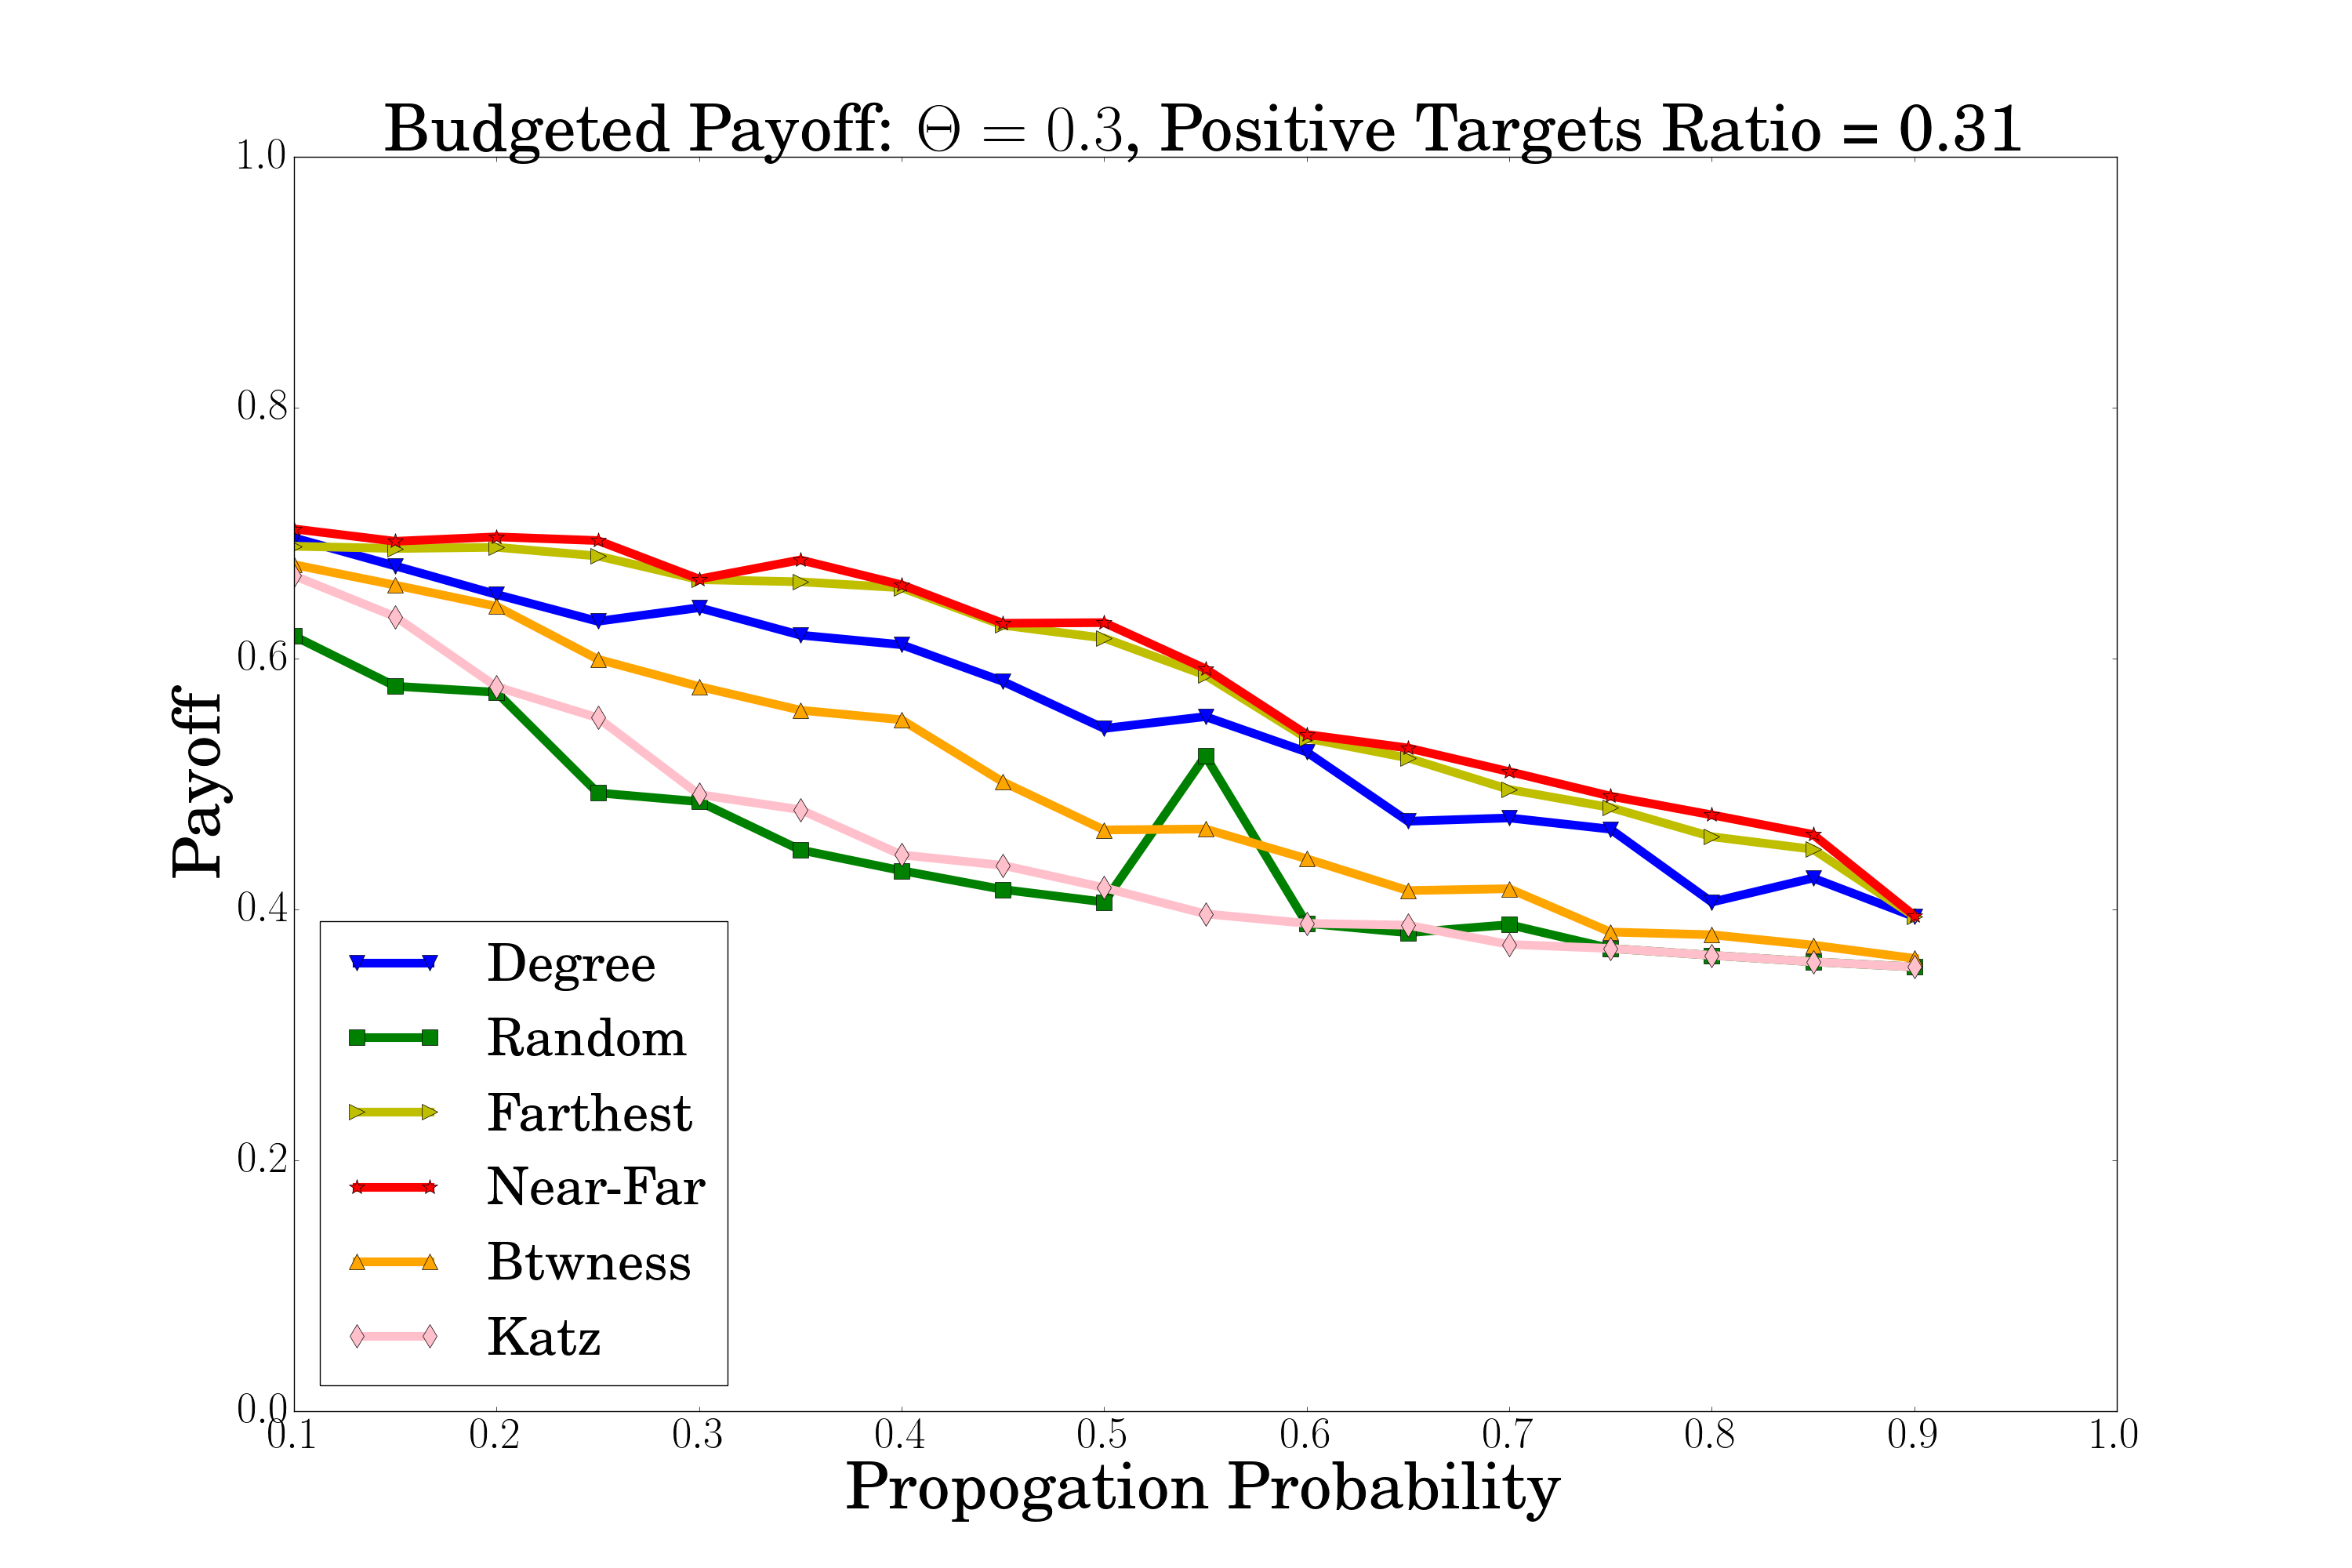
\includegraphics[width=1\textwidth]{../plots/budgeted/theta=3.png}
  \end{subfigure}\par\medskip
  \begin{subfigure}{\linewidth}
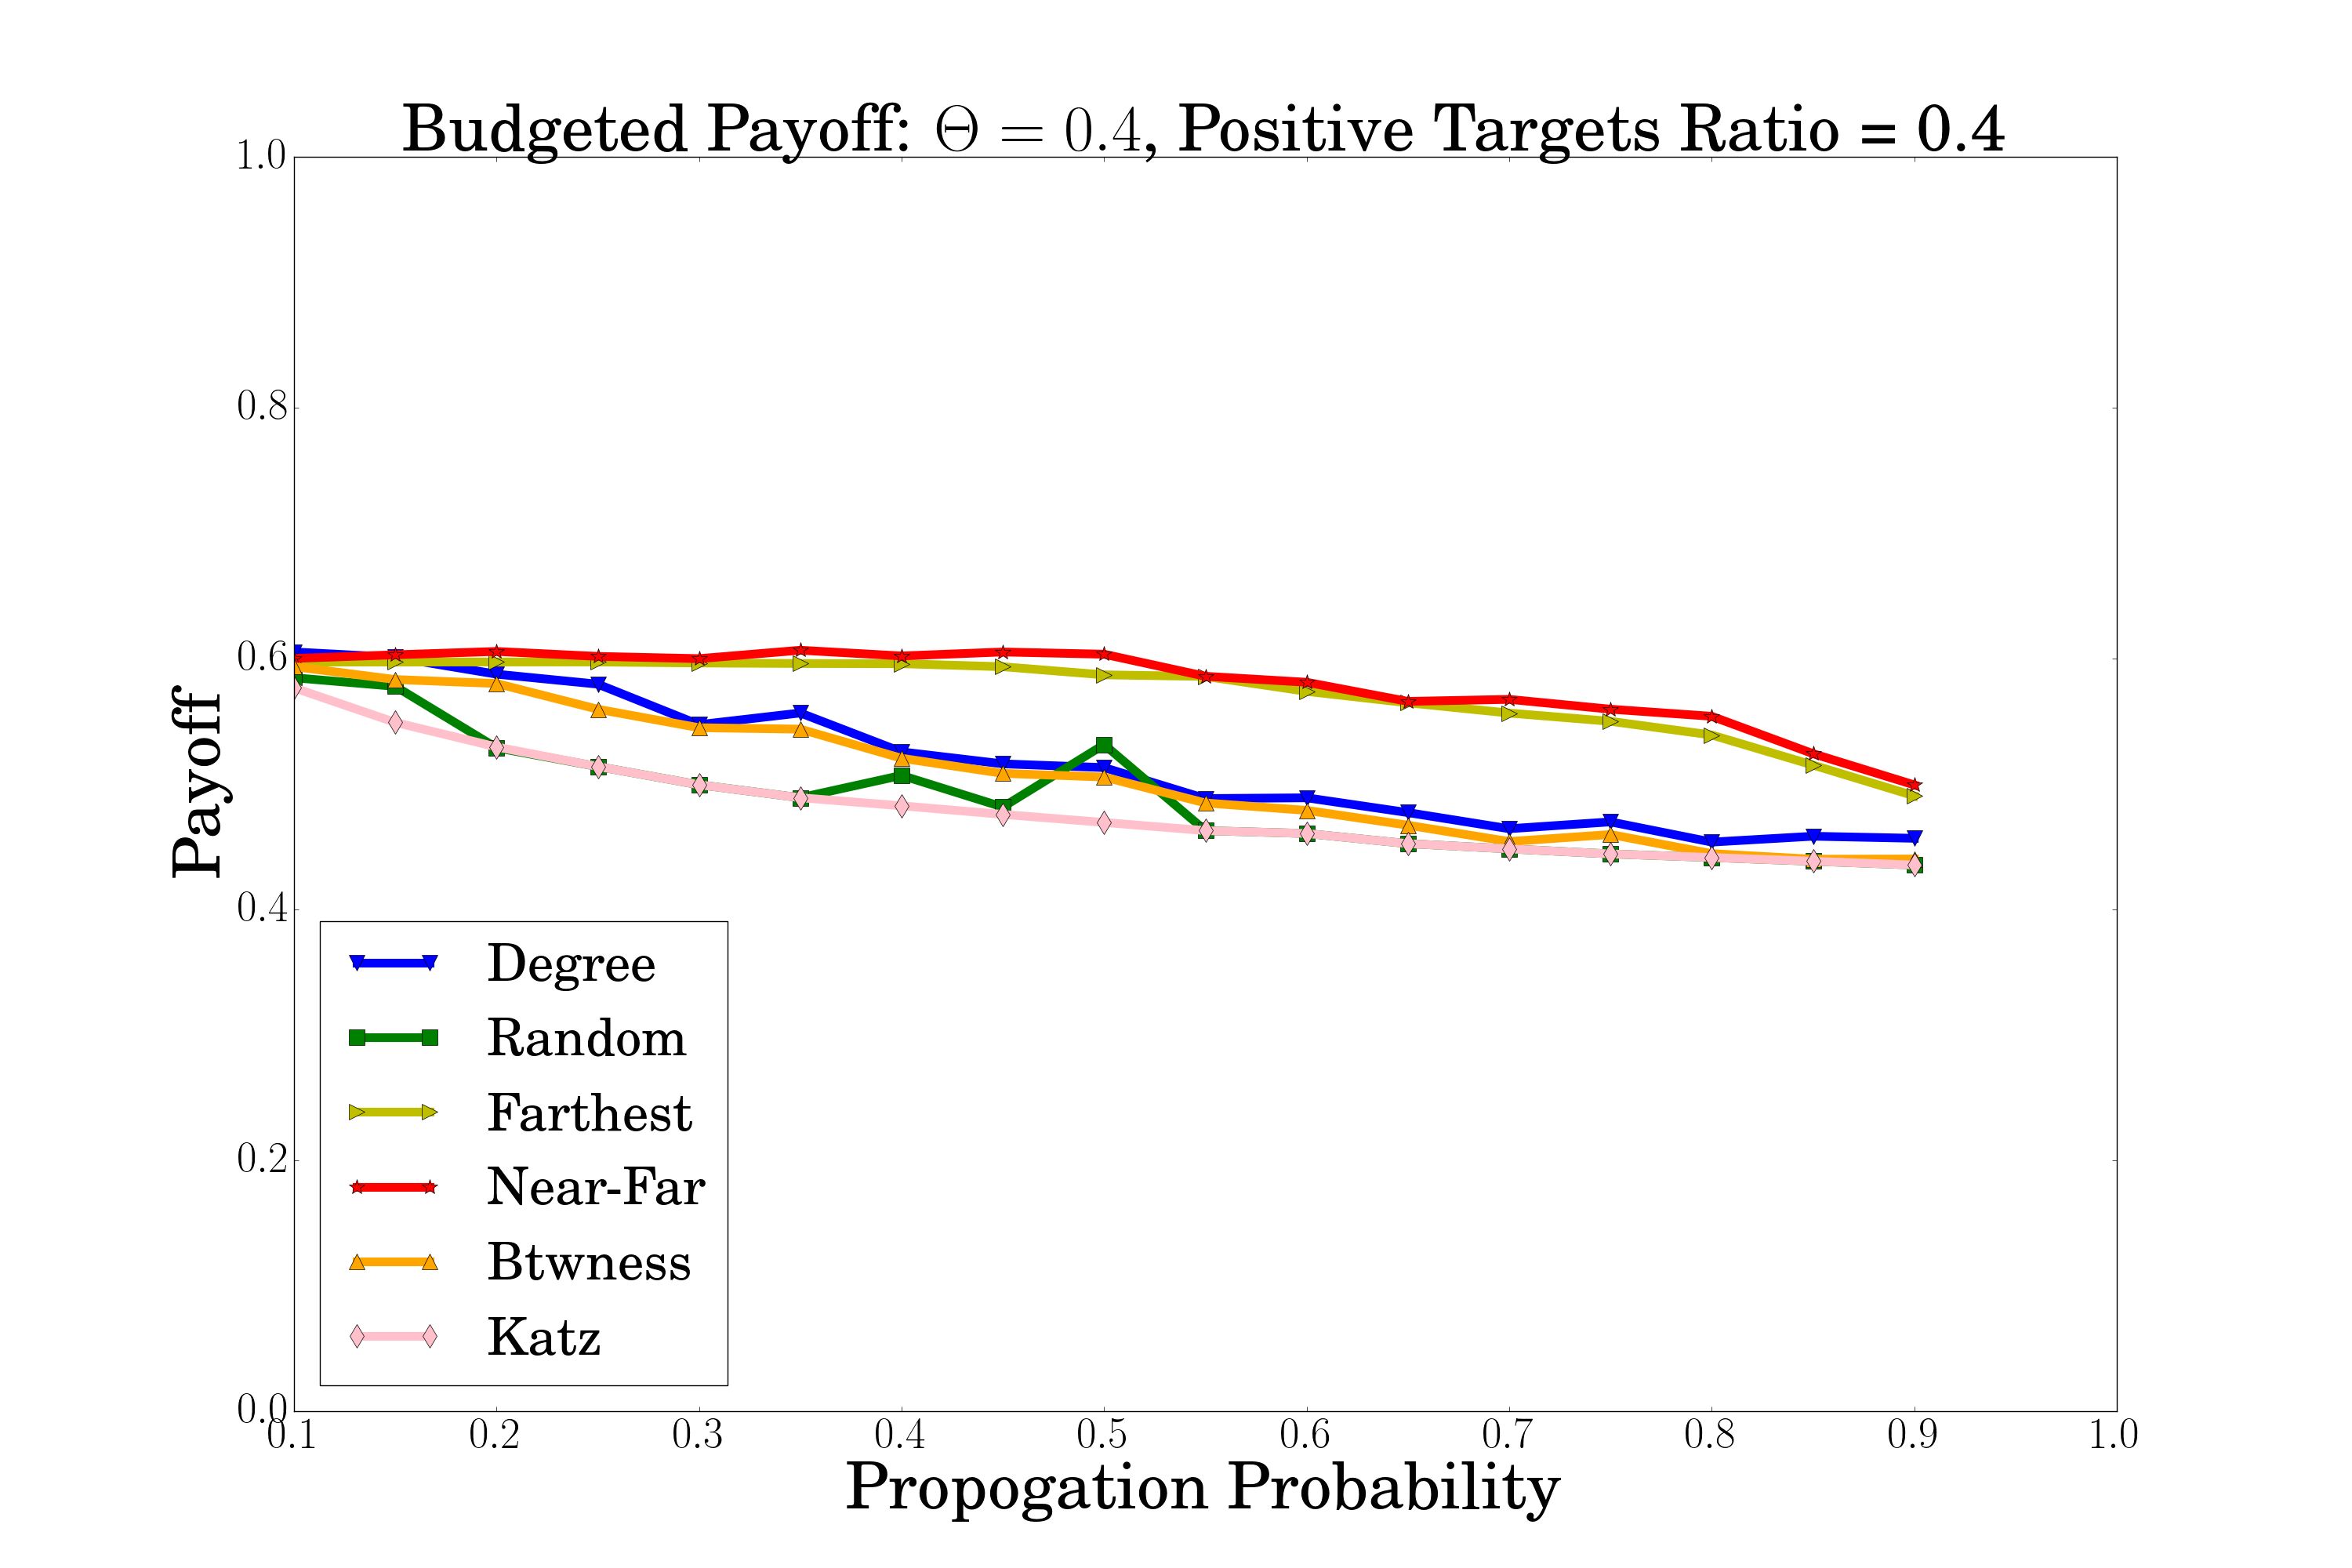
\includegraphics[width=1\textwidth]{../plots/budgeted/theta=4.png}
  \end{subfigure}\par\medskip
  %  \caption{Heuristic Results when $\theta$ < 0.5}
%\end{figure}
  
%\begin{figure}
  \begin{subfigure}{\linewidth}
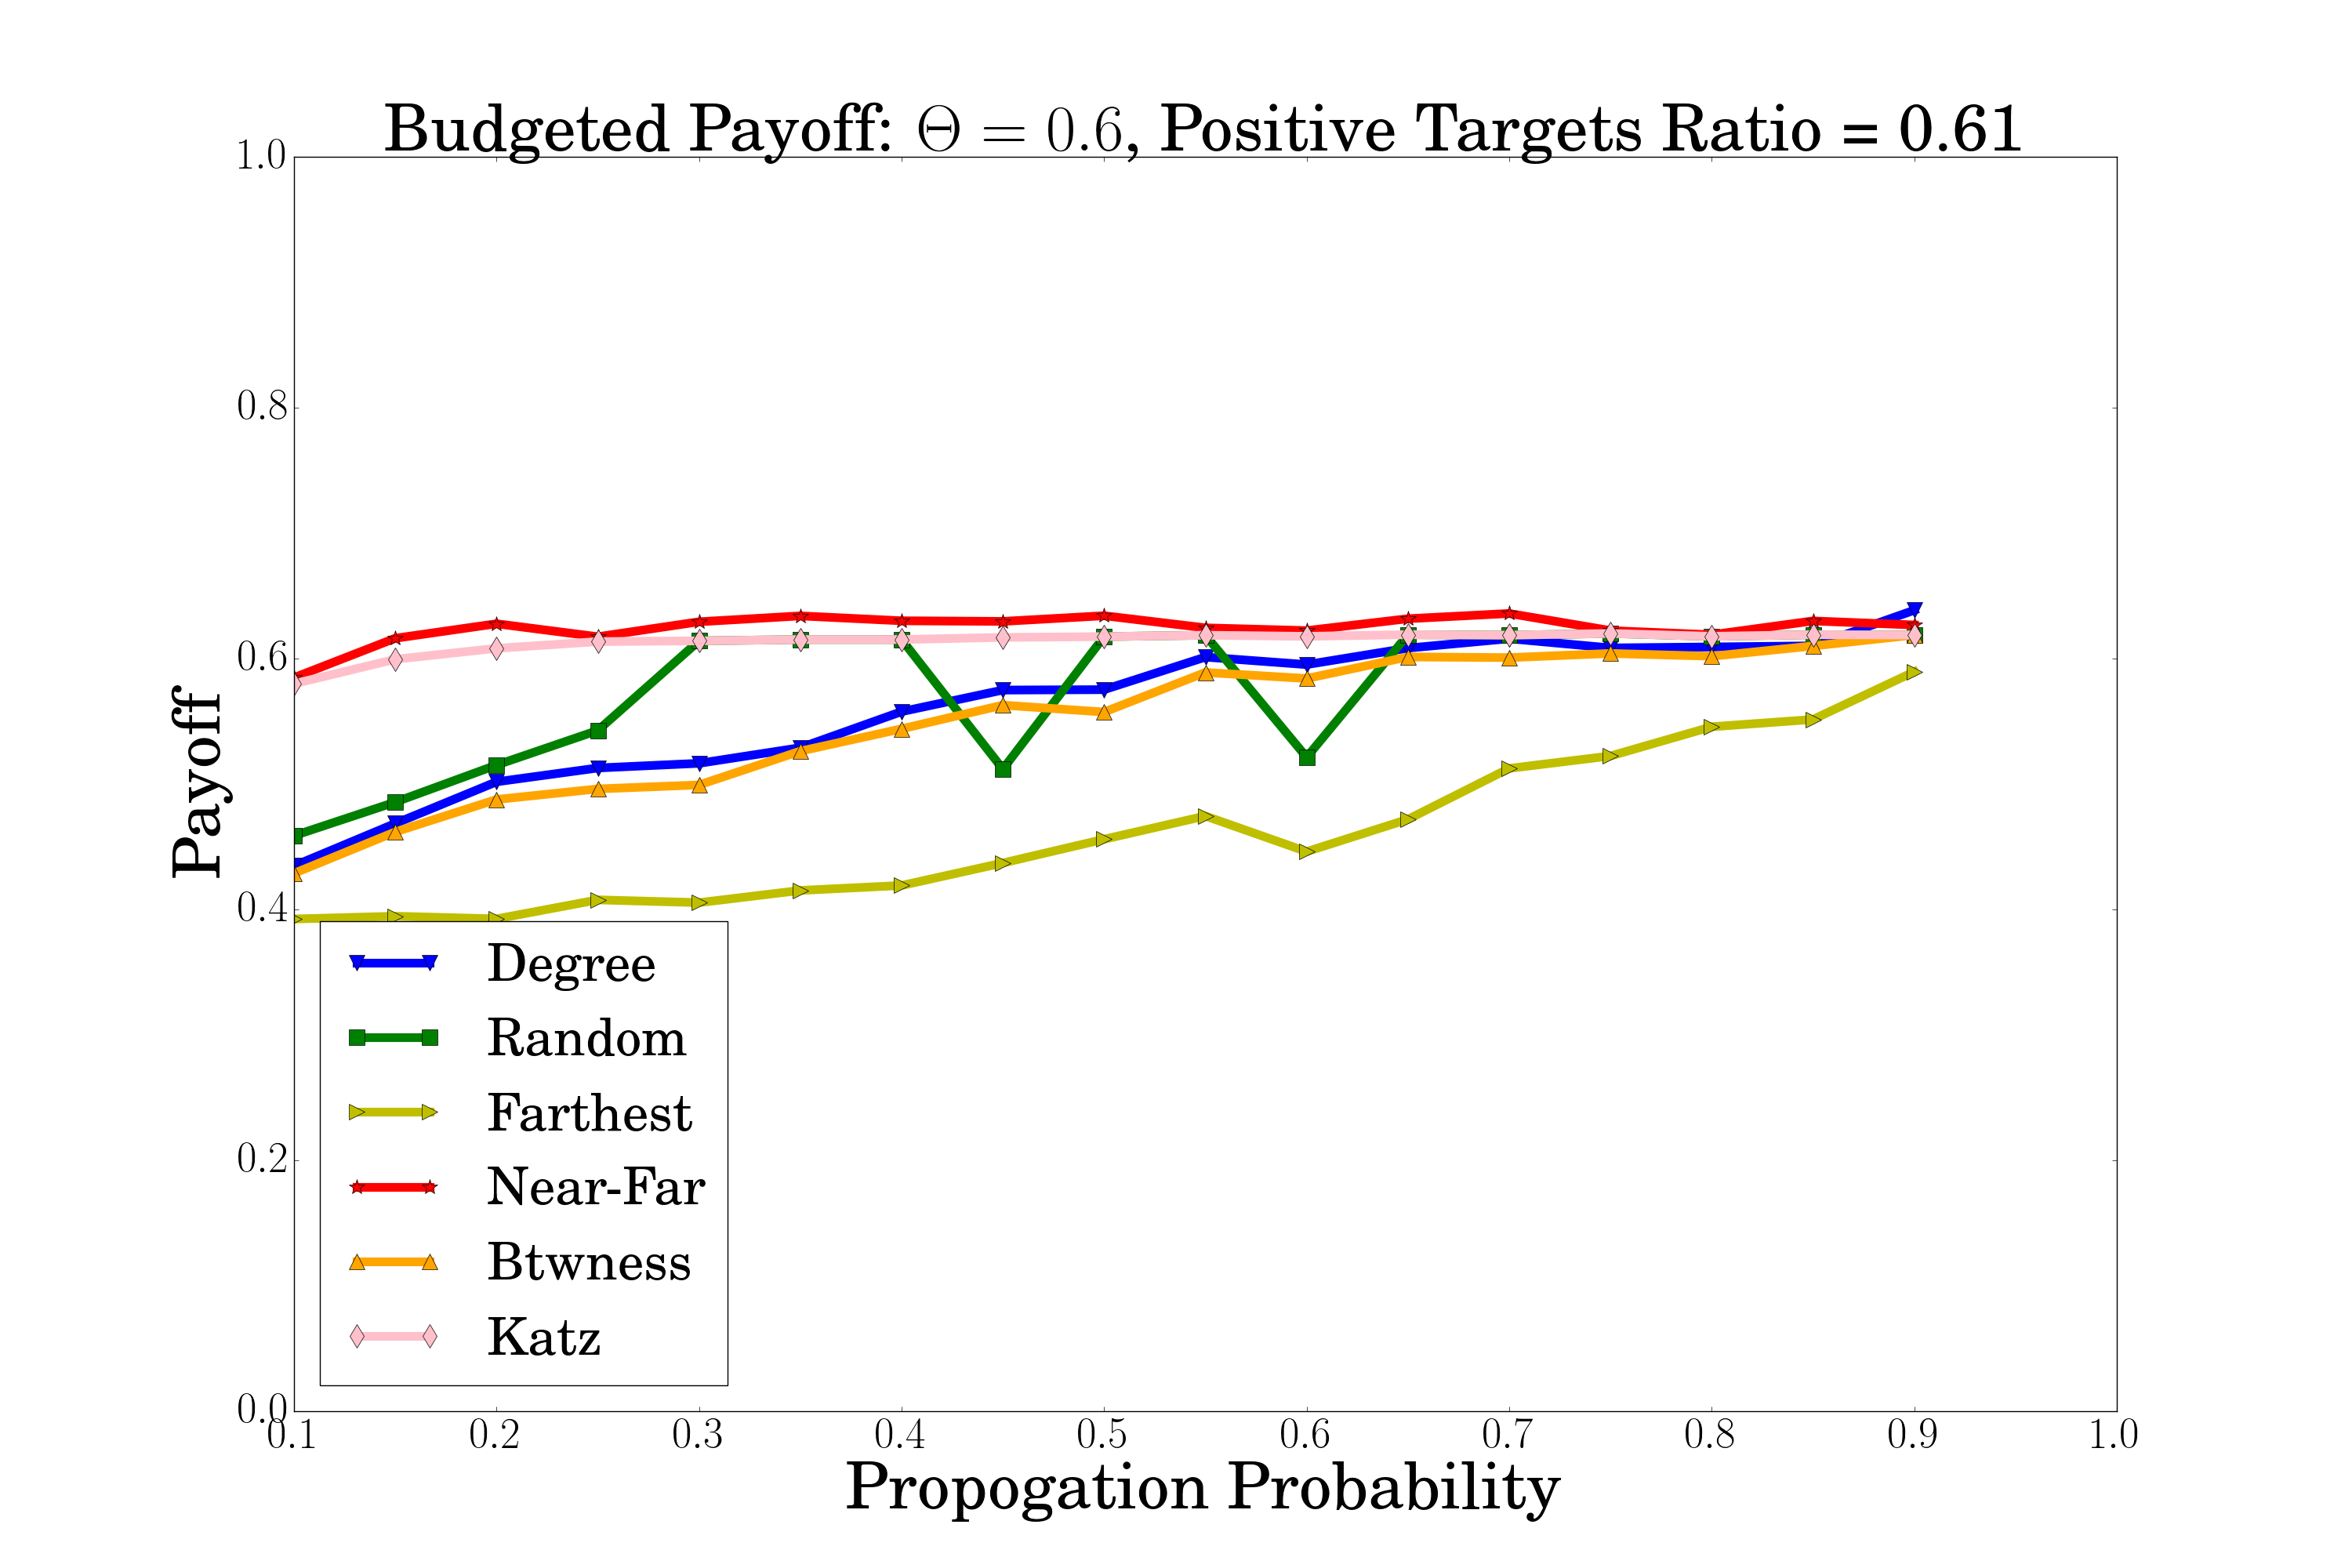
\includegraphics[width=1\textwidth]{../plots/budgeted/theta=6.png}
  \end{subfigure}
   \begin{subfigure}{\linewidth}
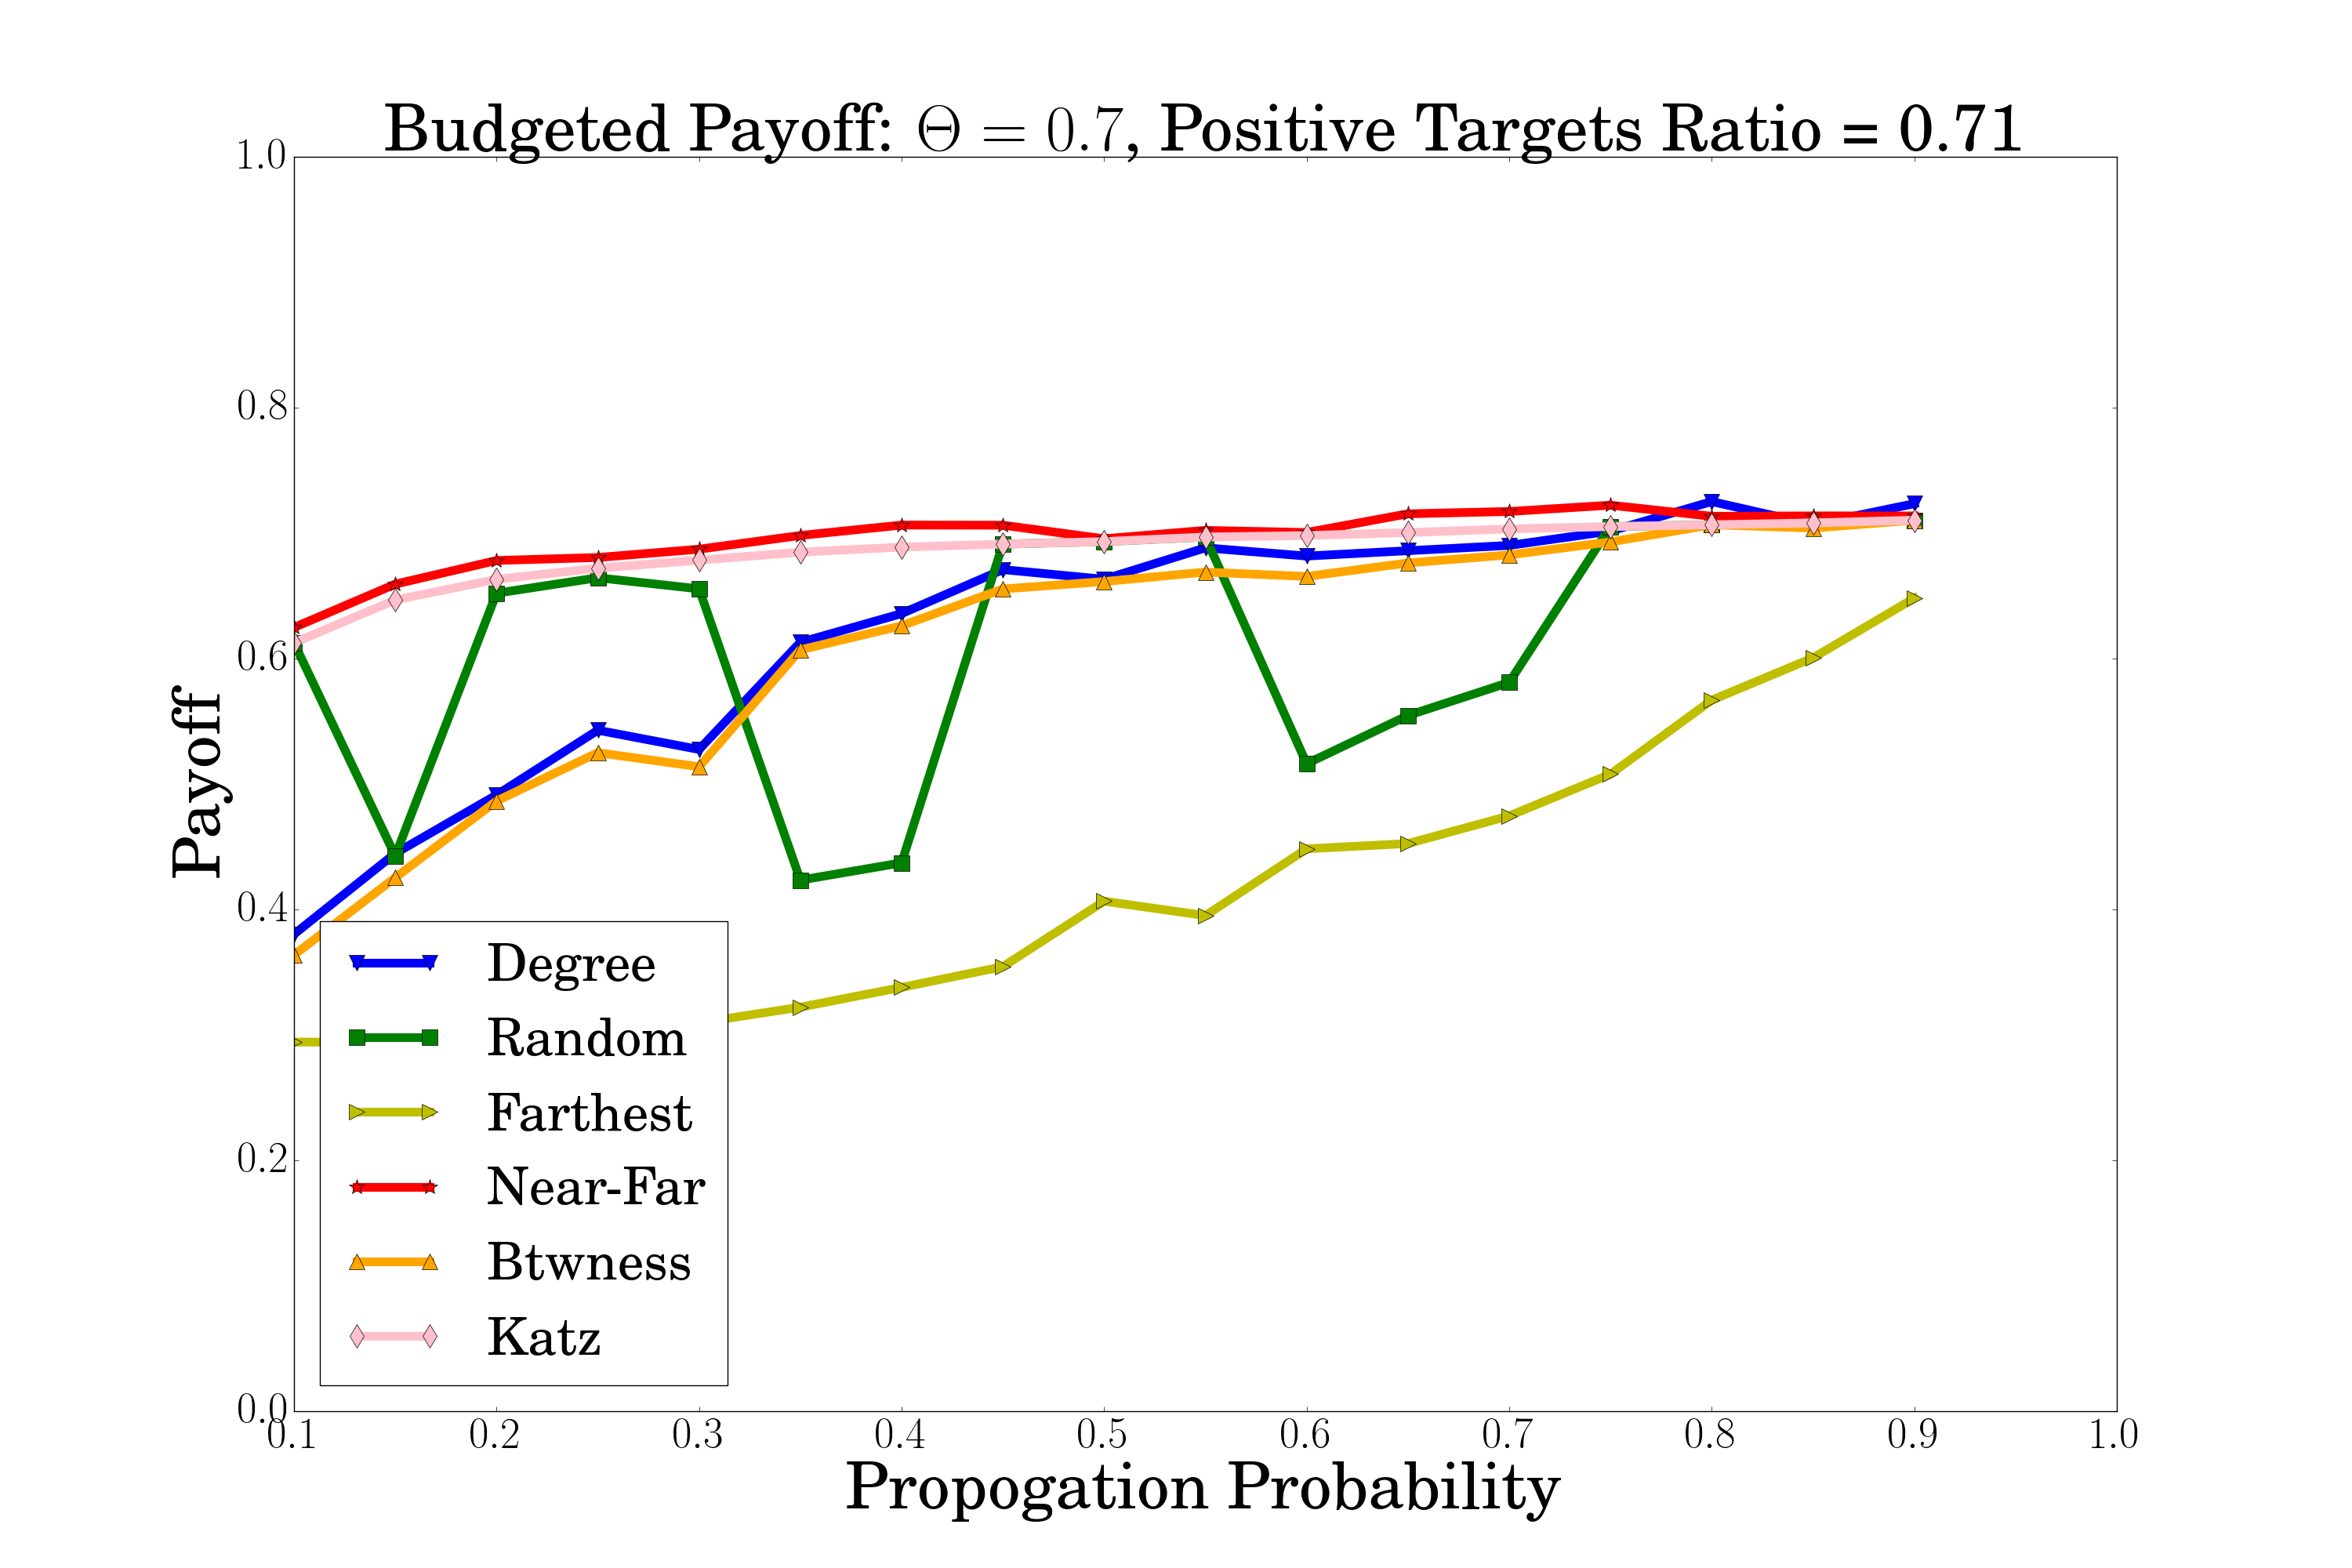
\includegraphics[width=1\textwidth]{../plots/budgeted/theta=7.png}
  \end{subfigure}
  \caption{Policy Budgeted Results}
\end{figure}

 \begin{figure}
  \begin{subfigure}{\linewidth}
  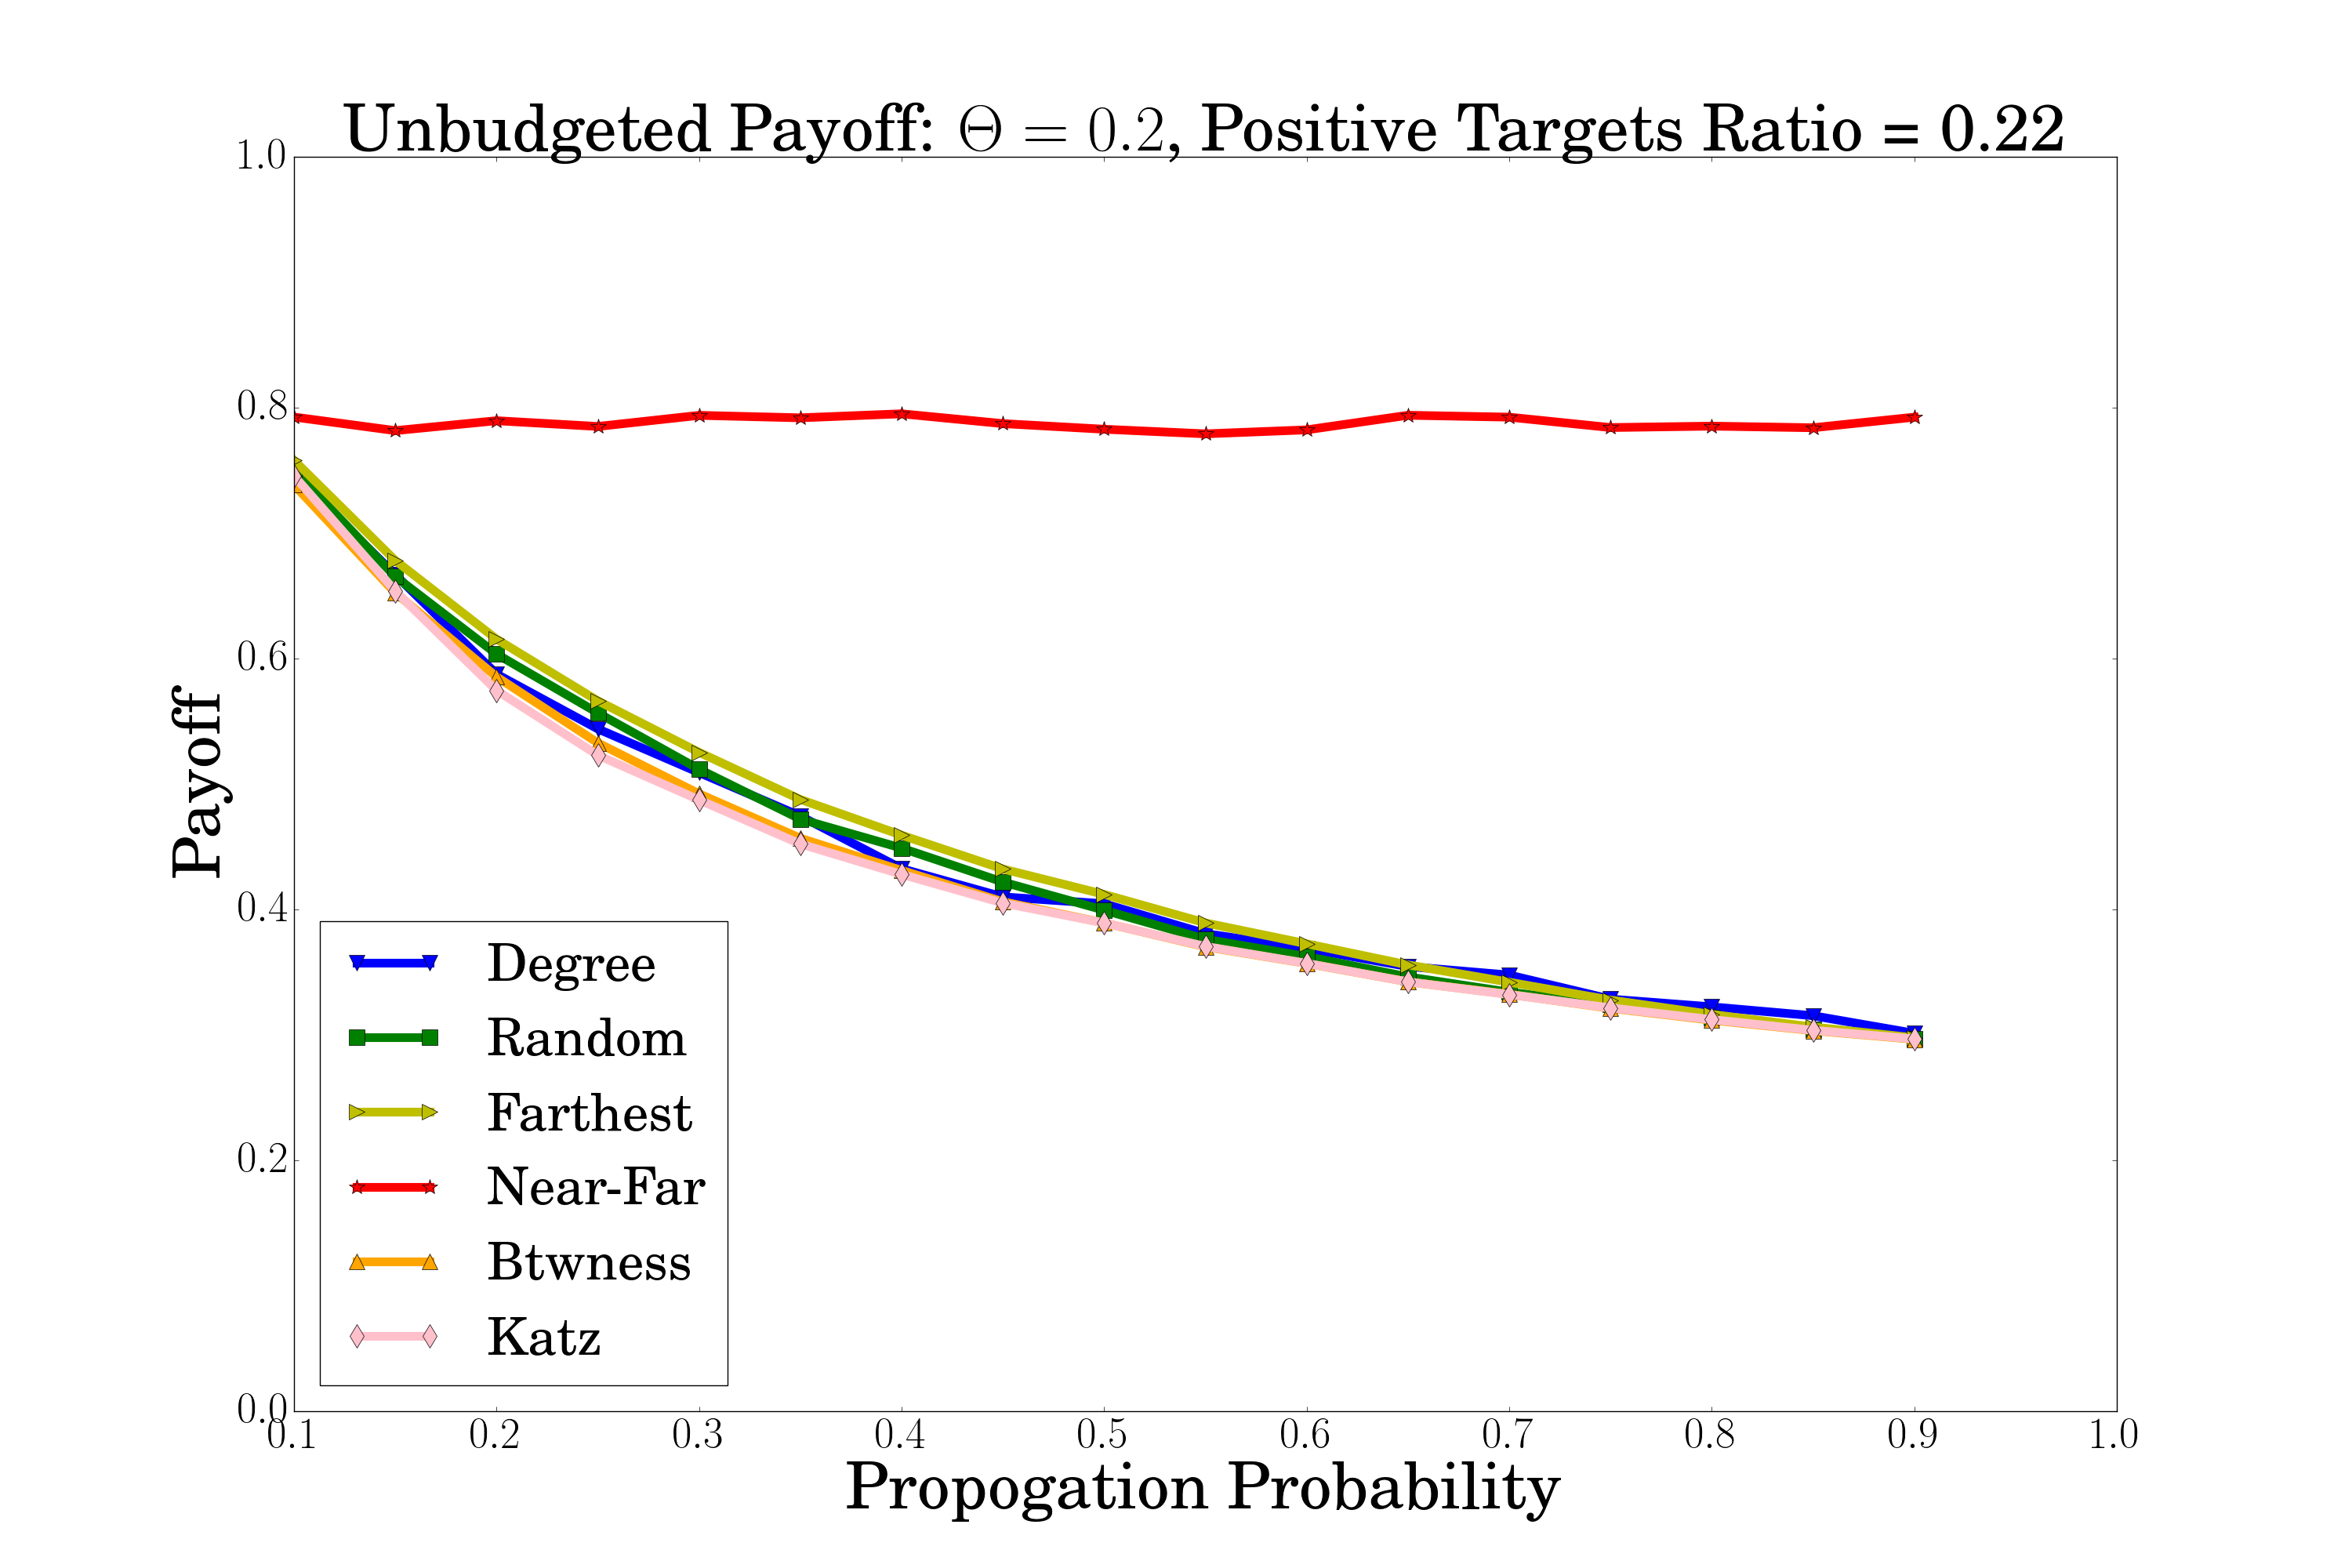
\includegraphics[width=1\textwidth]{../plots/unbudgeted/theta=2.png}
  \end{subfigure}\par\medskip
  \begin{subfigure}{\linewidth}
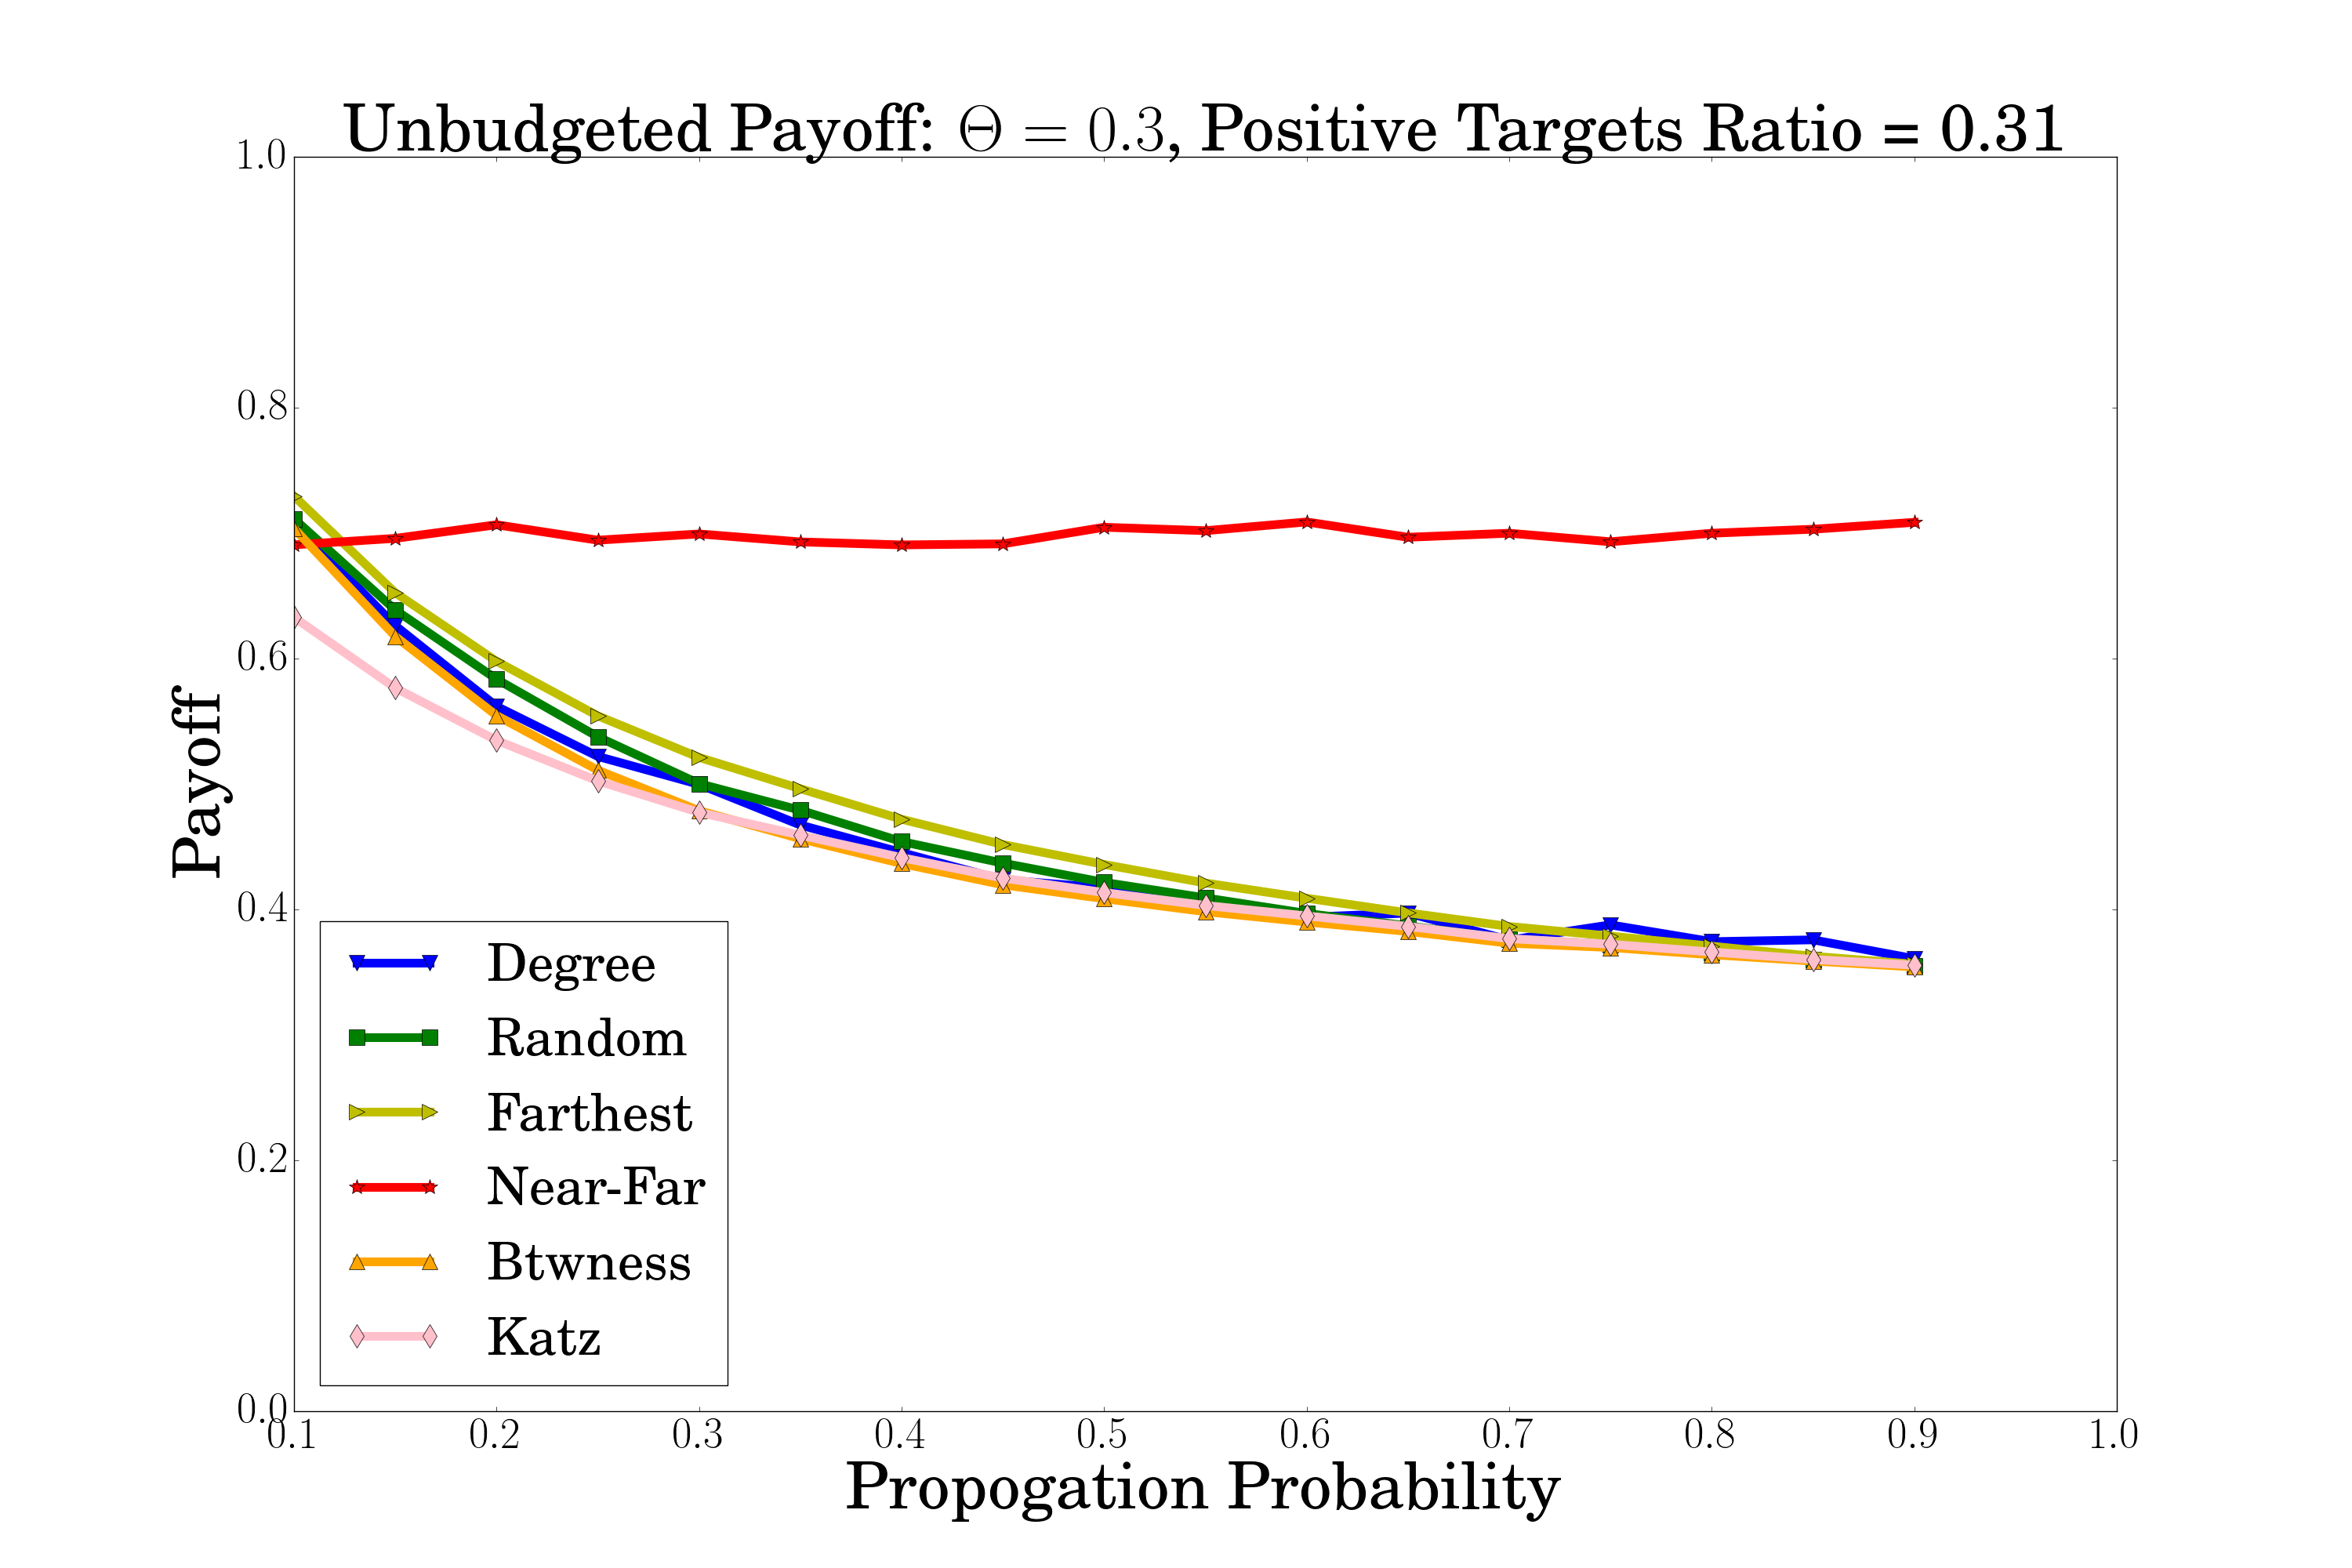
\includegraphics[width=1\textwidth]{../plots/unbudgeted/theta=3.png}
  \end{subfigure}\par\medskip
  %  \caption{Heuristic Results when $\theta$ < 0.5}
%\end{figure}
  
%\begin{figure}
  \begin{subfigure}{\linewidth}
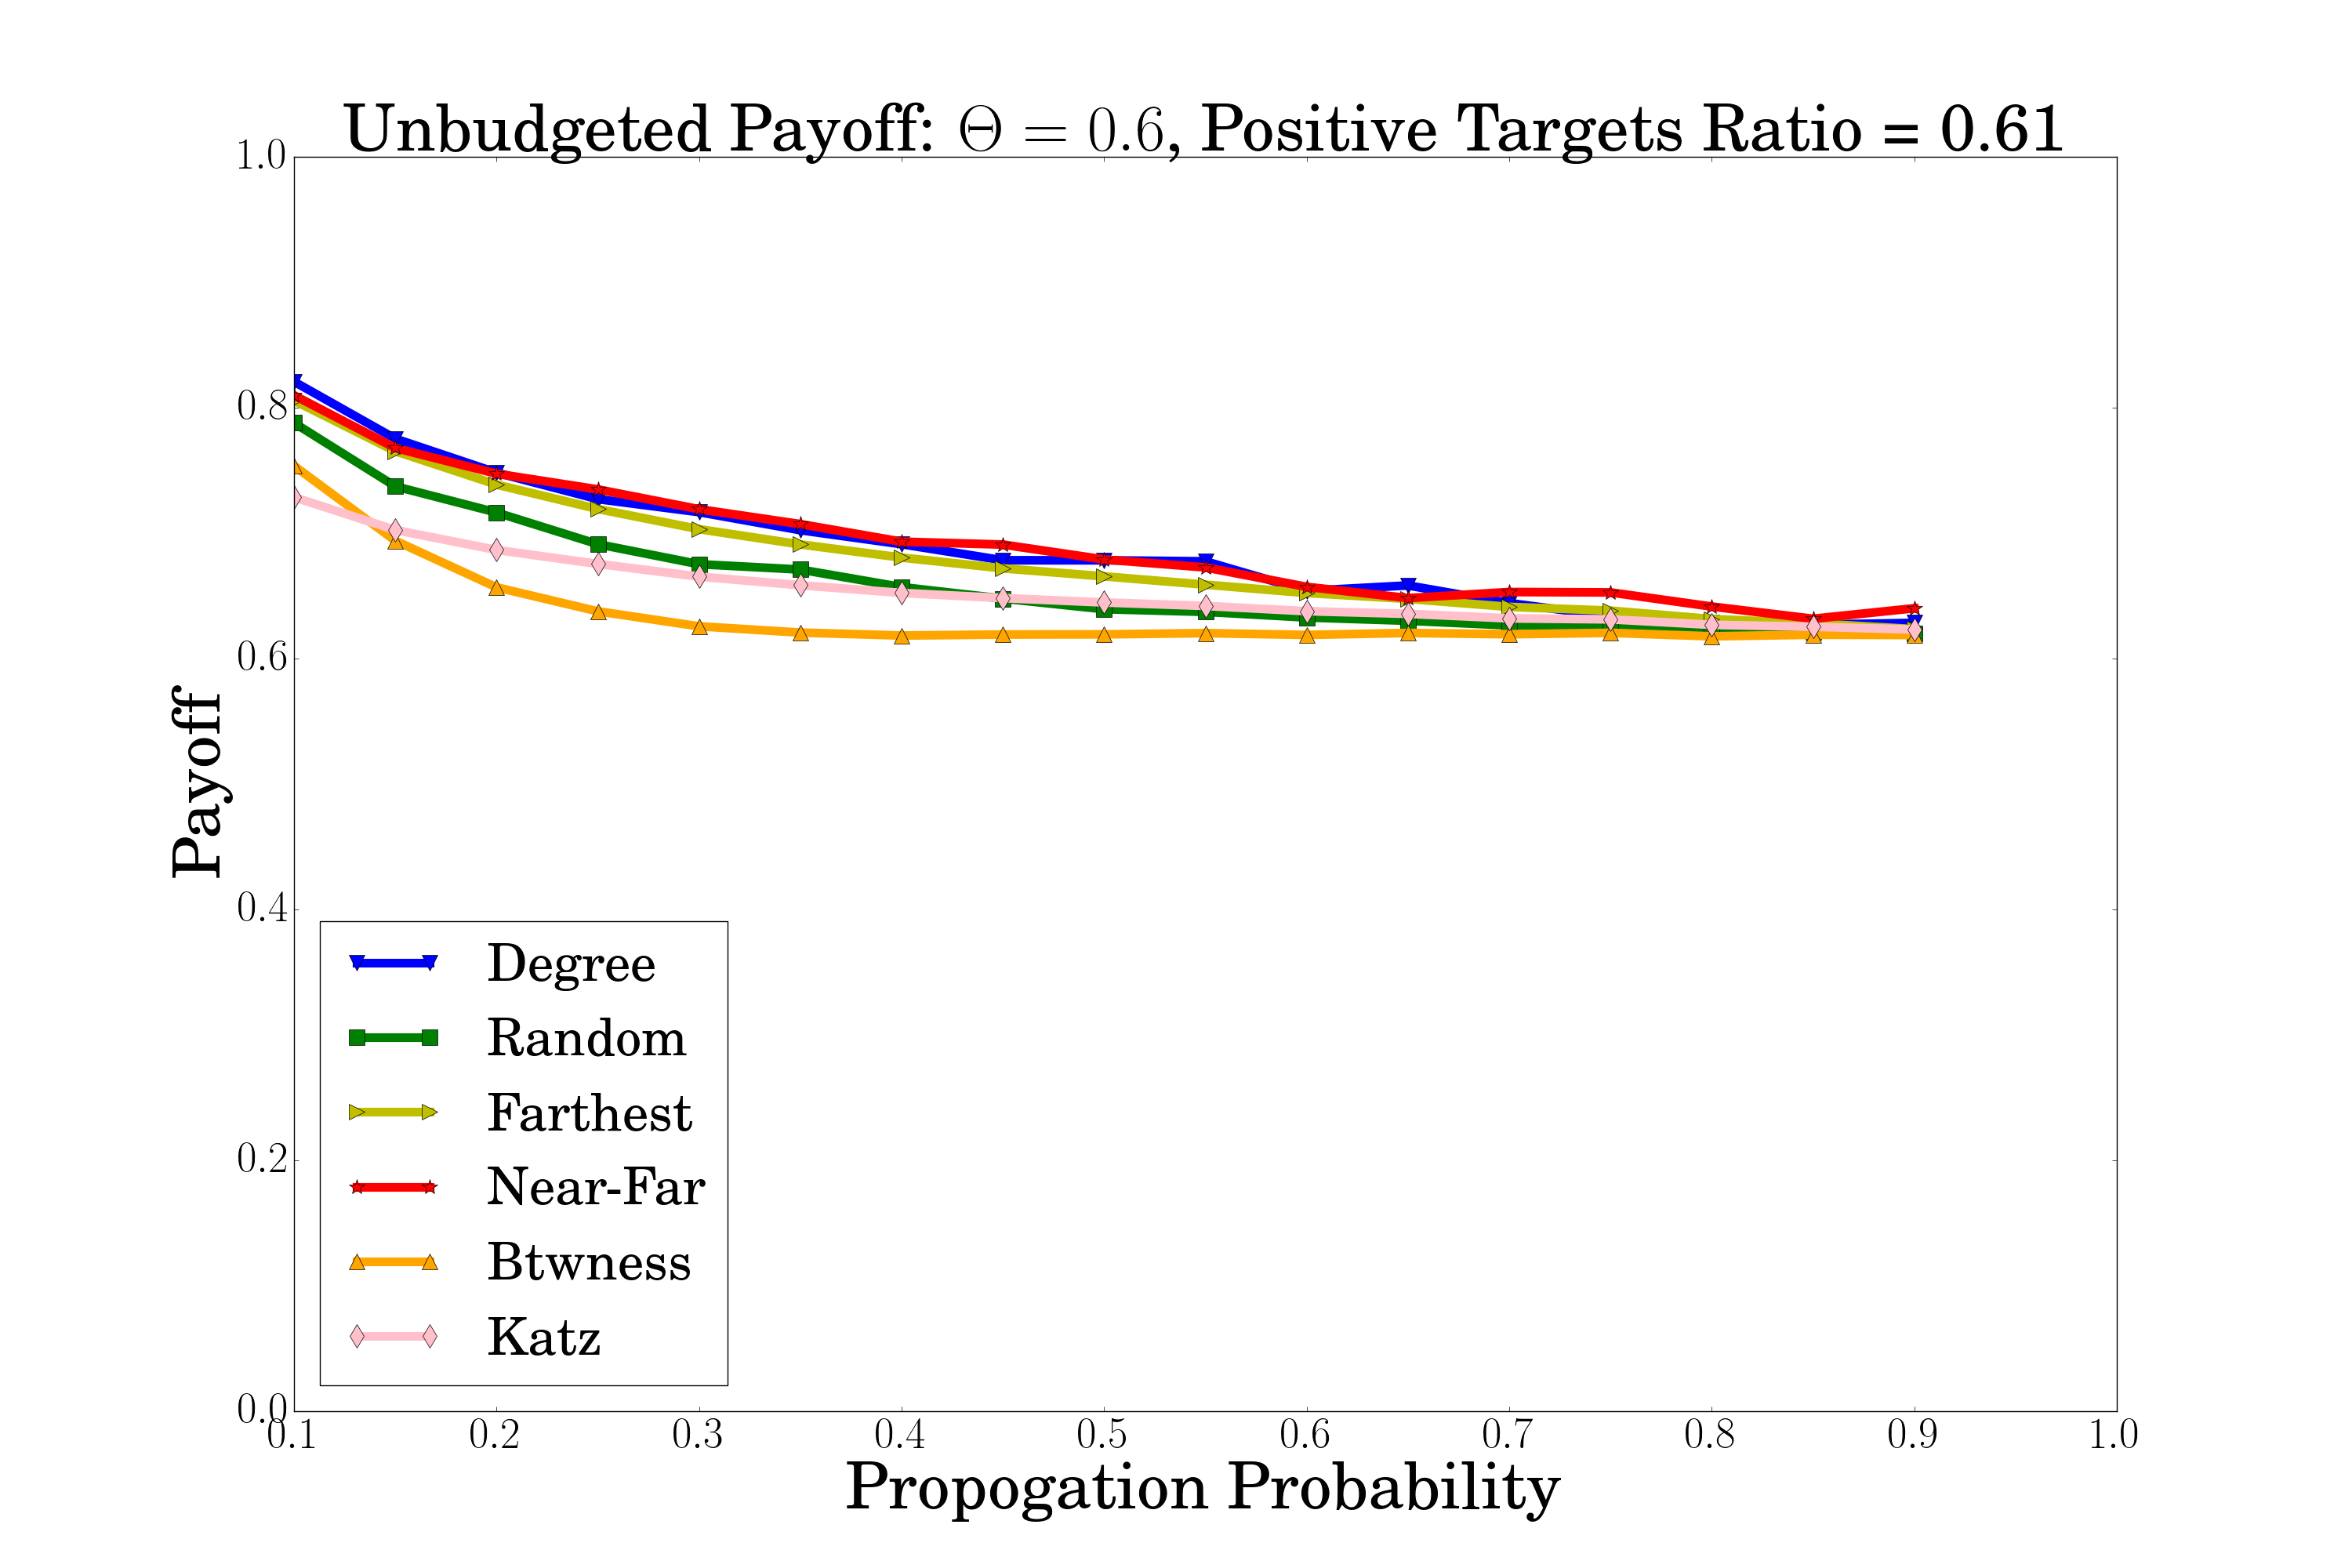
\includegraphics[width=1\textwidth]{../plots/unbudgeted/theta=6.png}
  \end{subfigure}
   \begin{subfigure}{\linewidth}
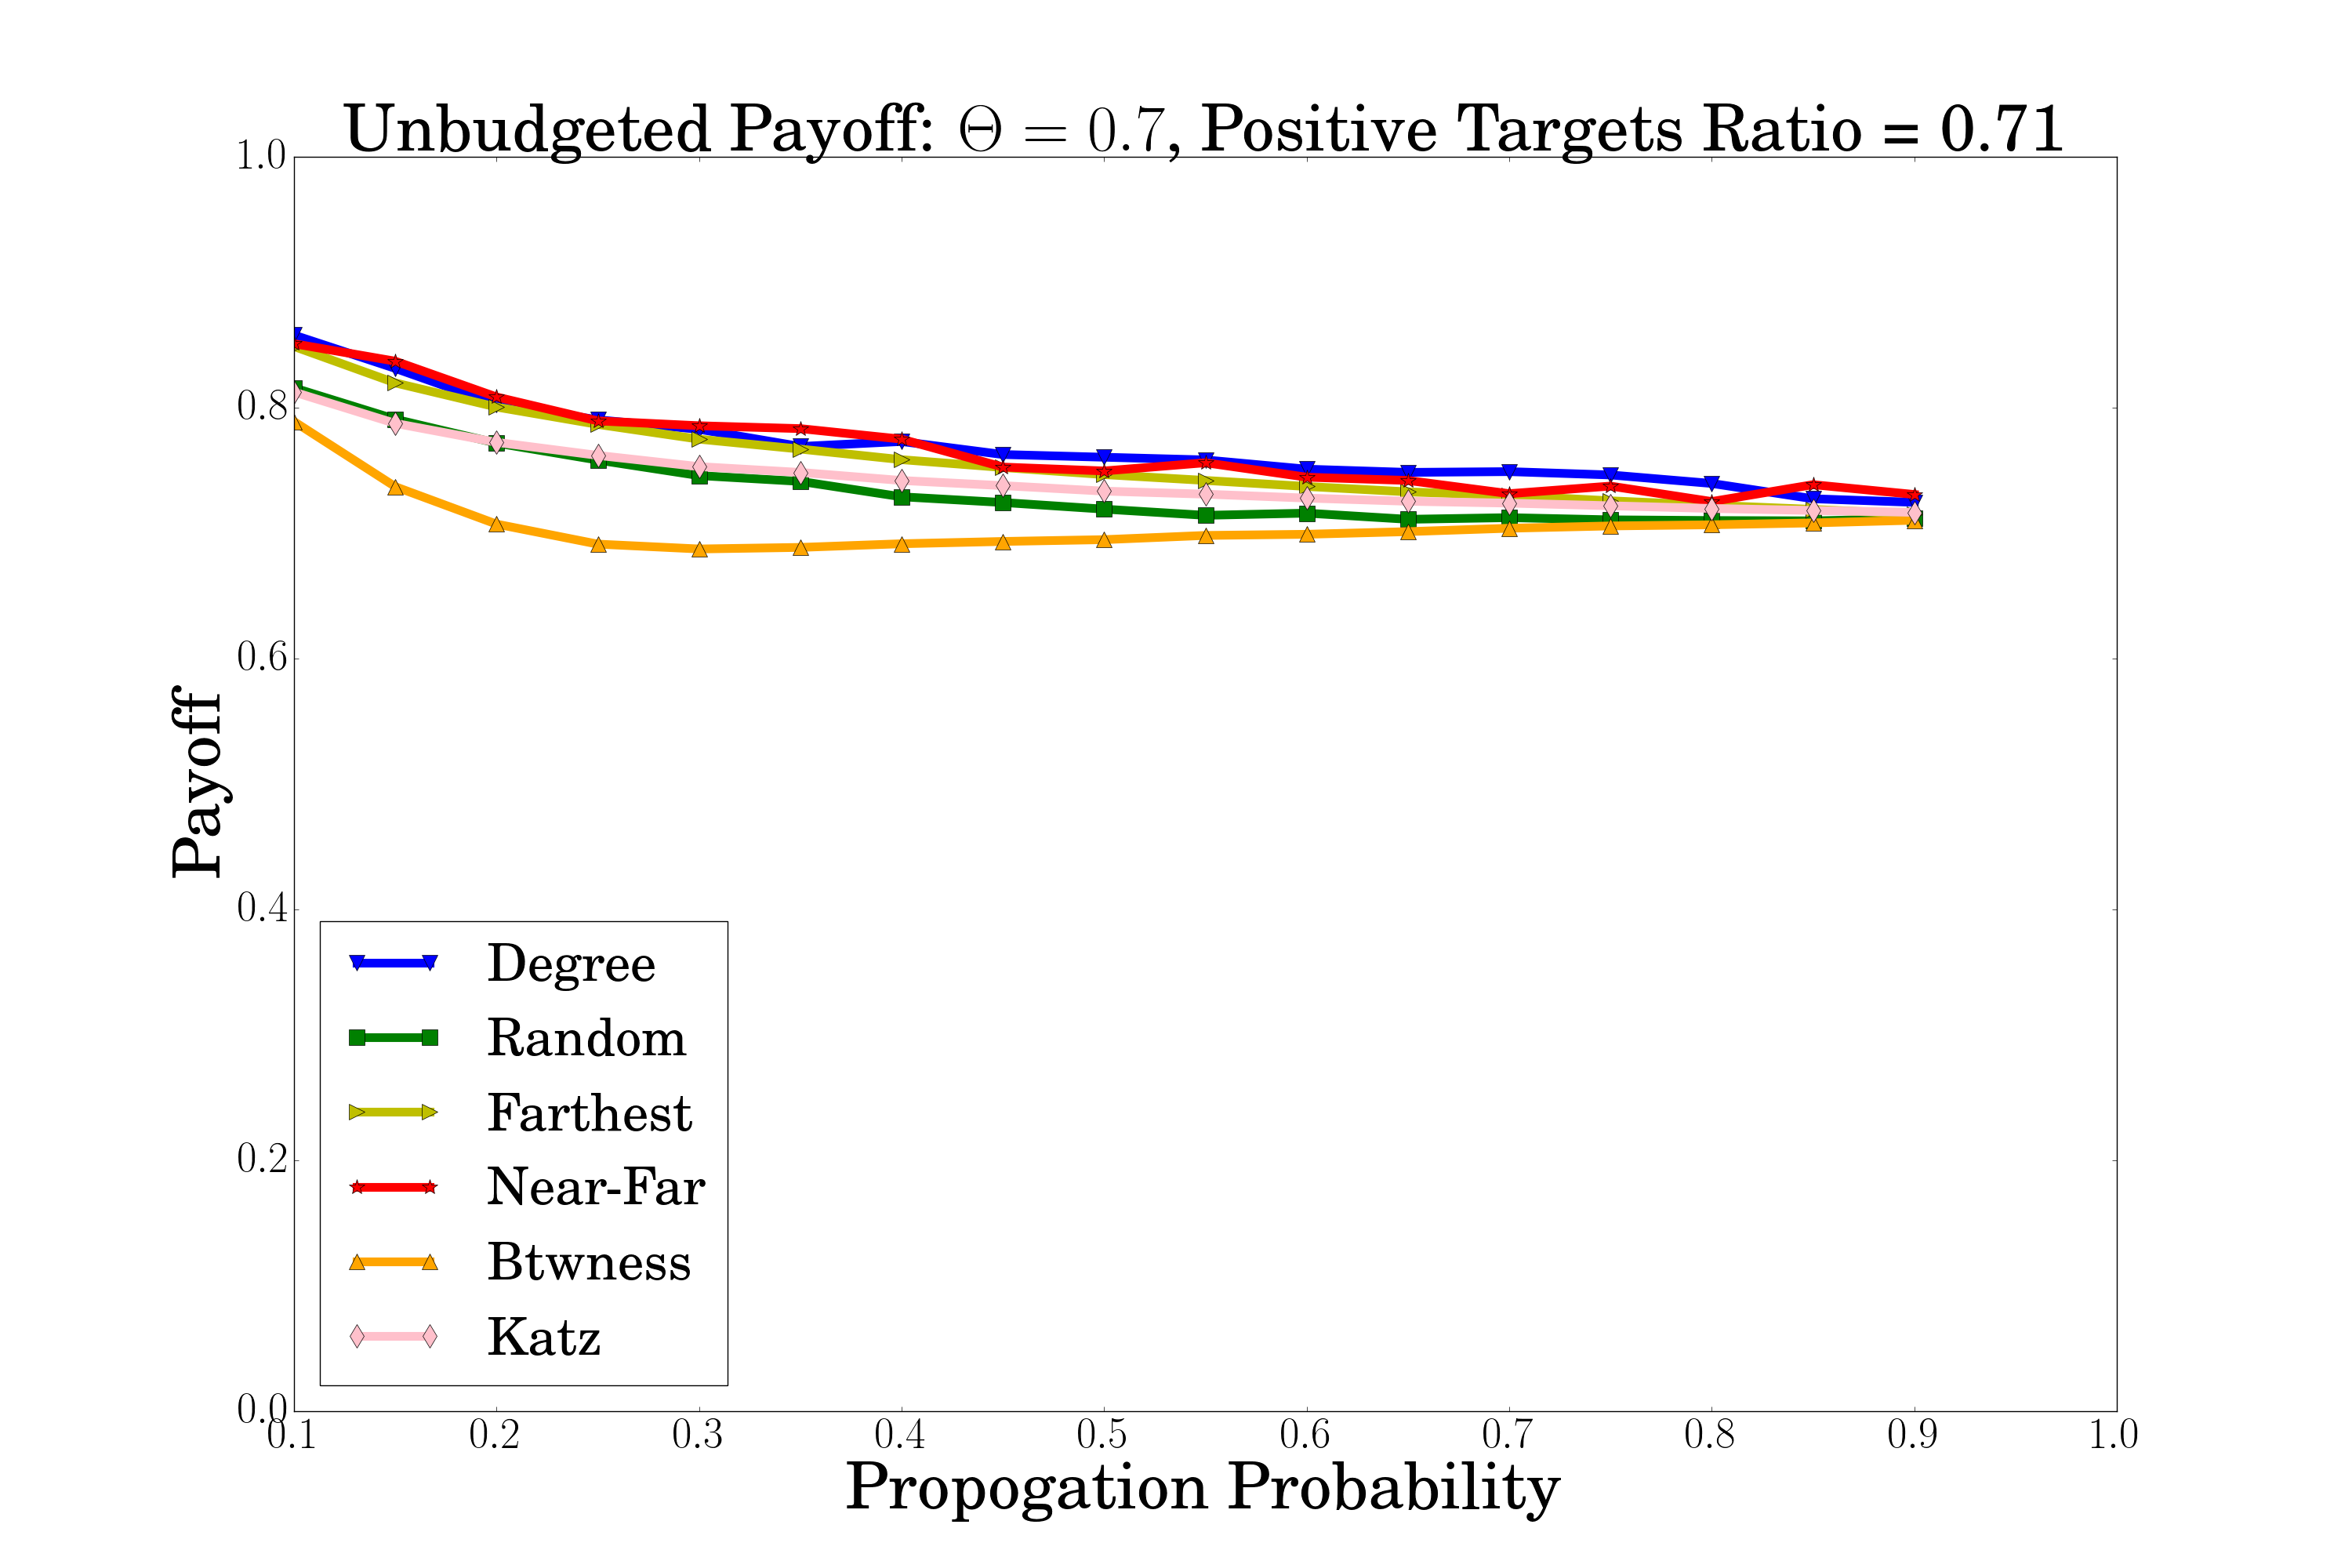
\includegraphics[width=1\textwidth]{../plots/unbudgeted/theta=7.png}
  \end{subfigure}
  \caption{Policy Unbudgeted Results}
\end{figure}

 \begin{figure}
  \begin{subfigure}{\linewidth}
  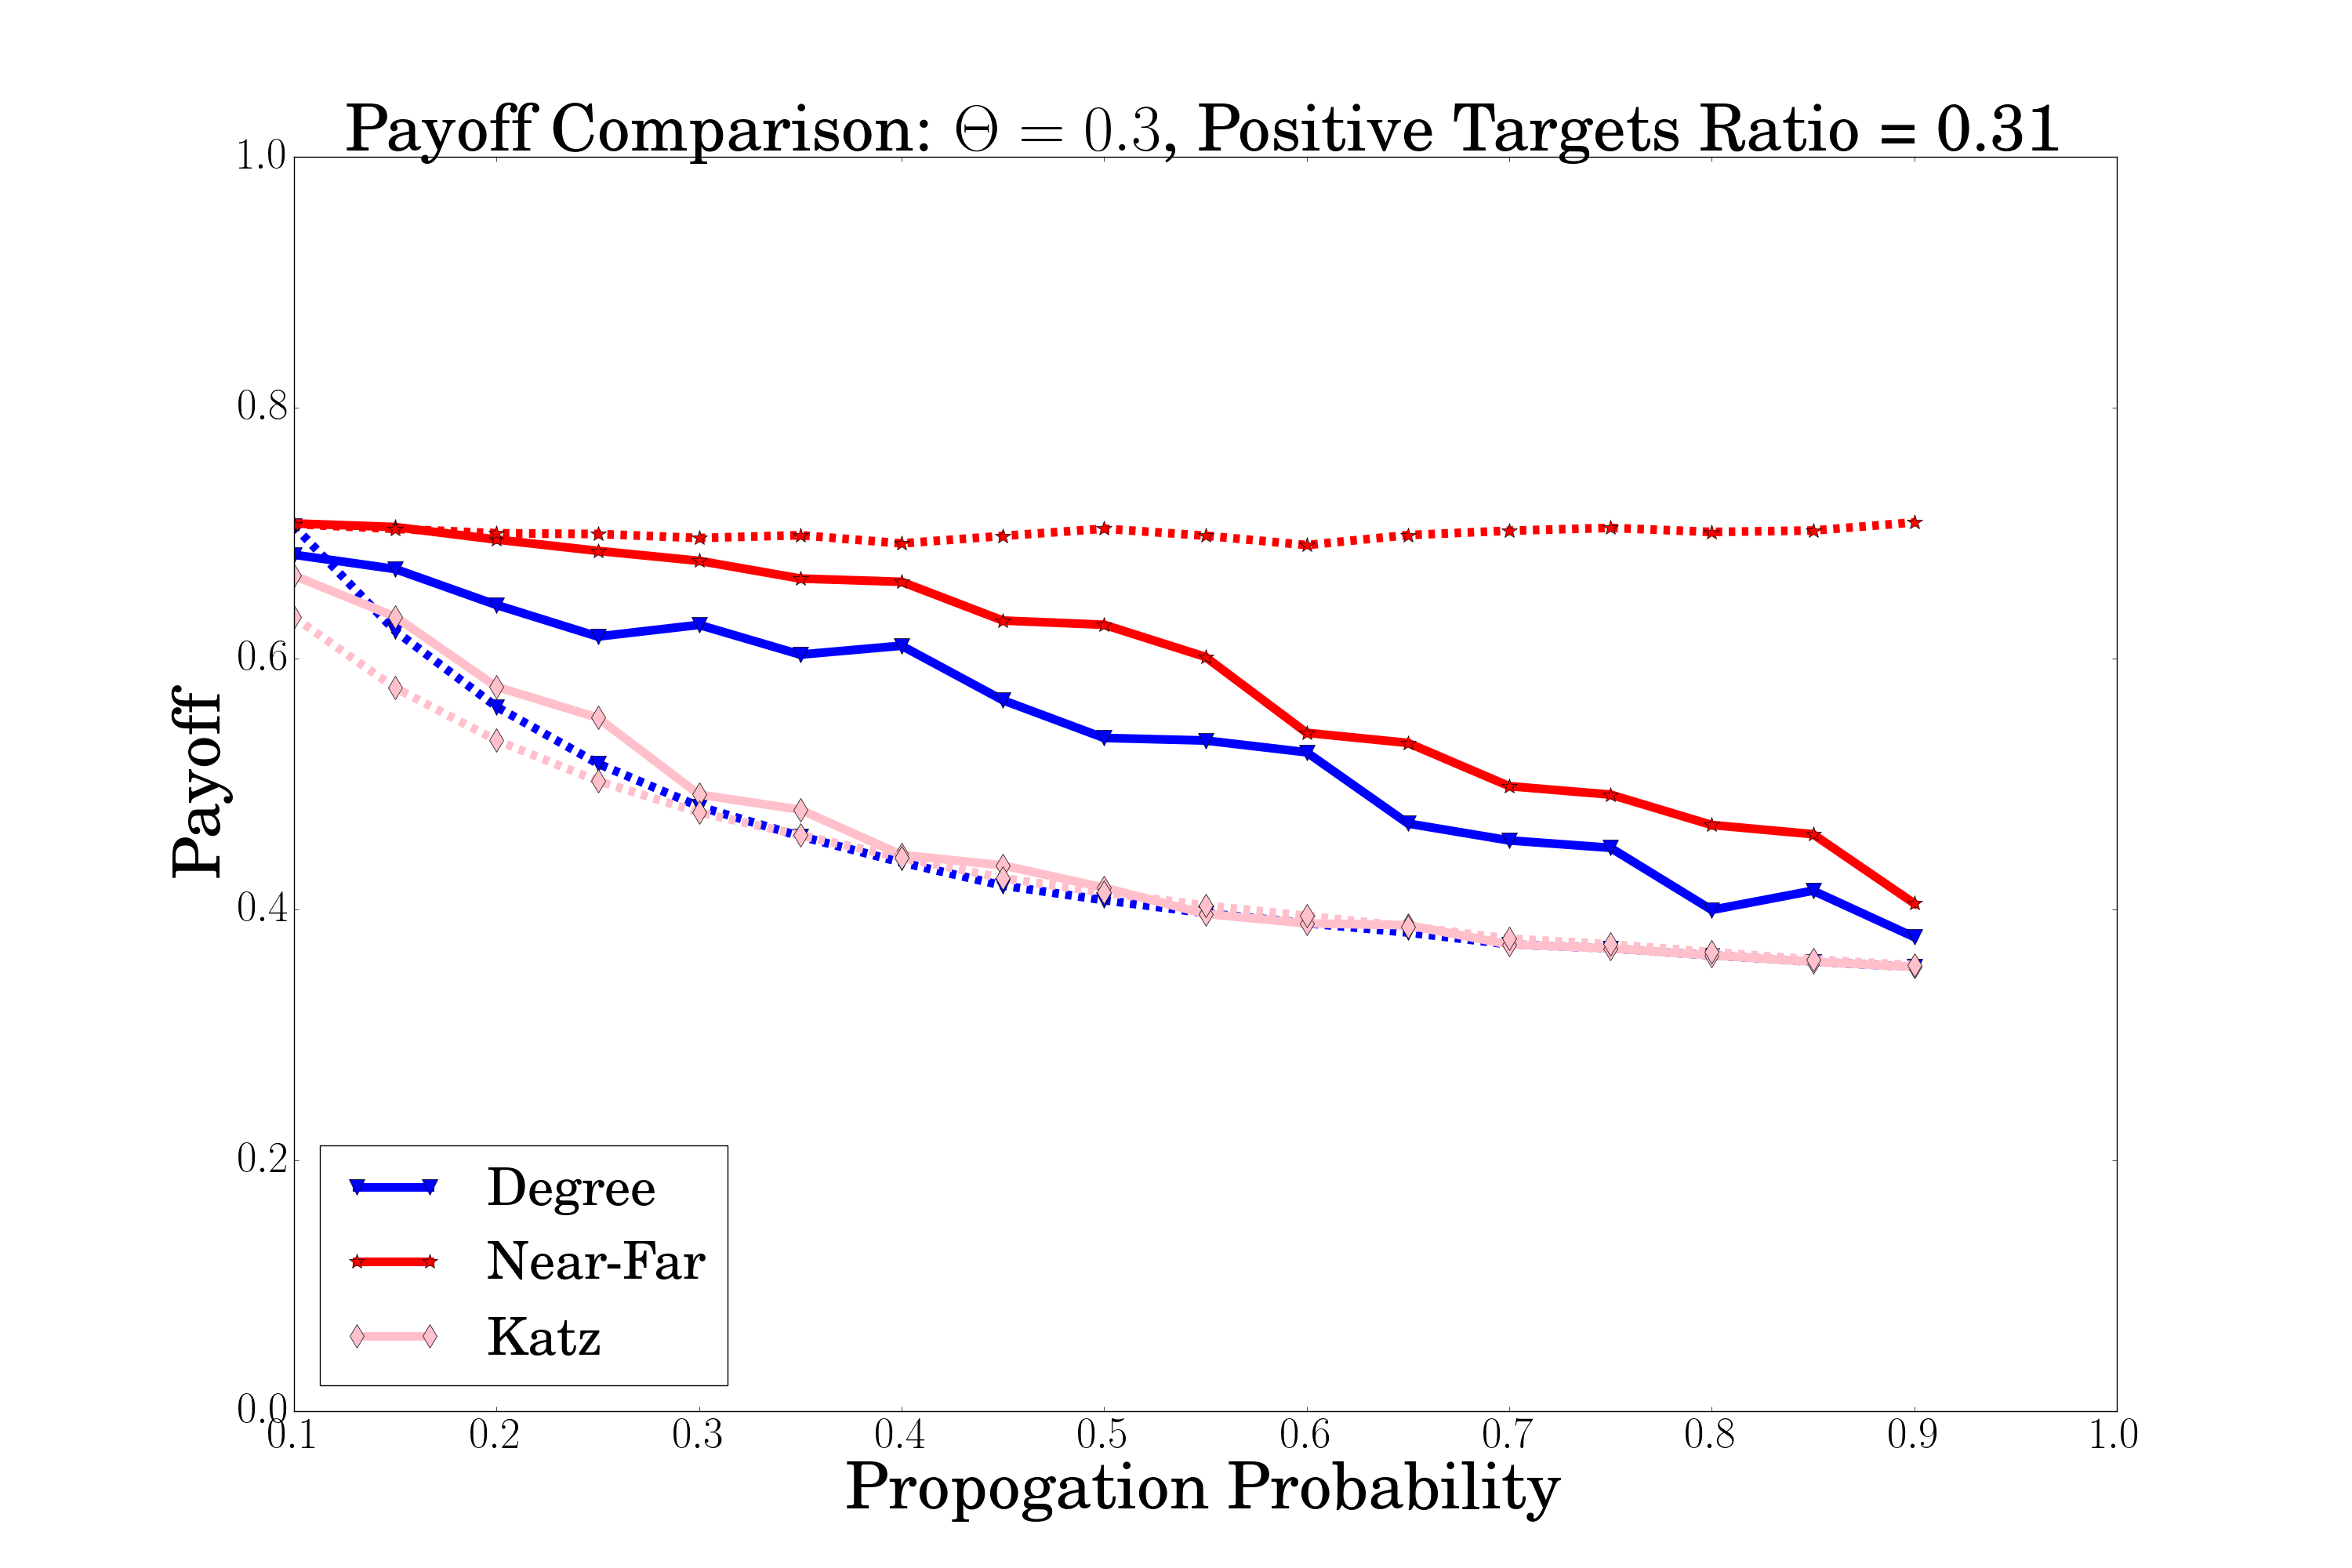
\includegraphics[width=1\textwidth]{../plots/comparison/theta=3.png}
  \end{subfigure}\par\medskip
  \begin{subfigure}{\linewidth}
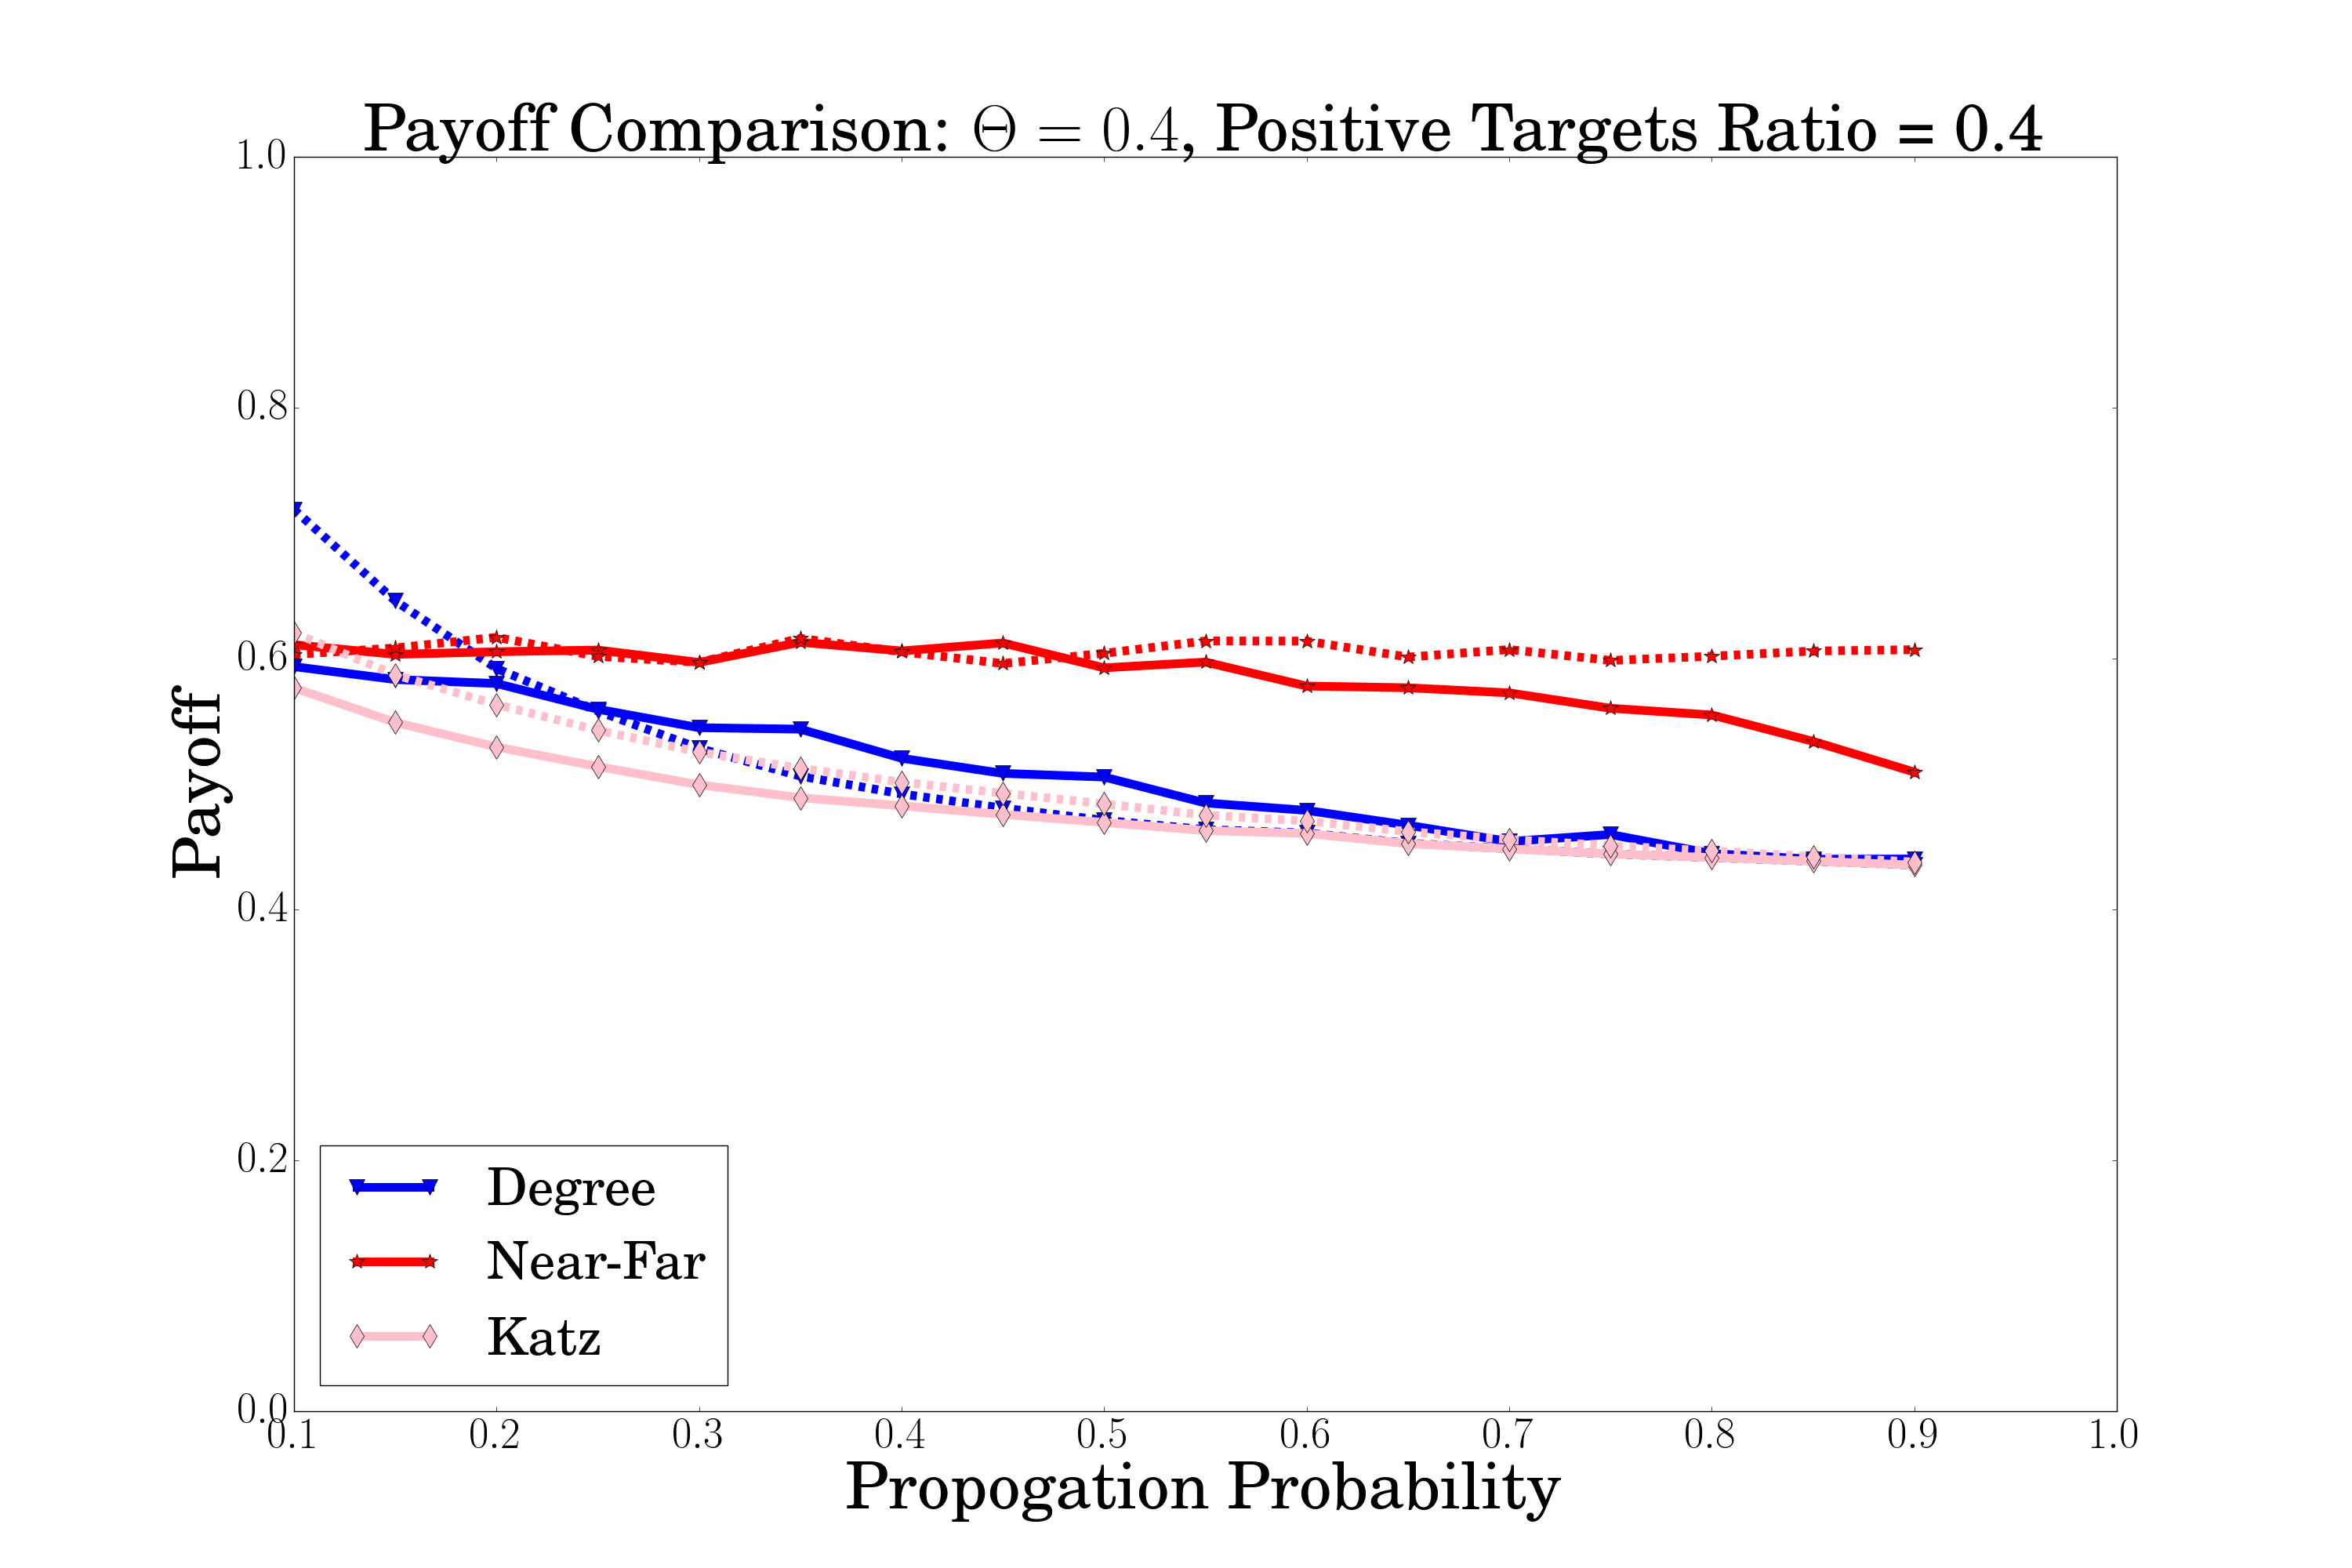
\includegraphics[width=1\textwidth]{../plots/comparison/theta=4.png}
  \end{subfigure}\par\medskip
    \begin{subfigure}{\linewidth}
  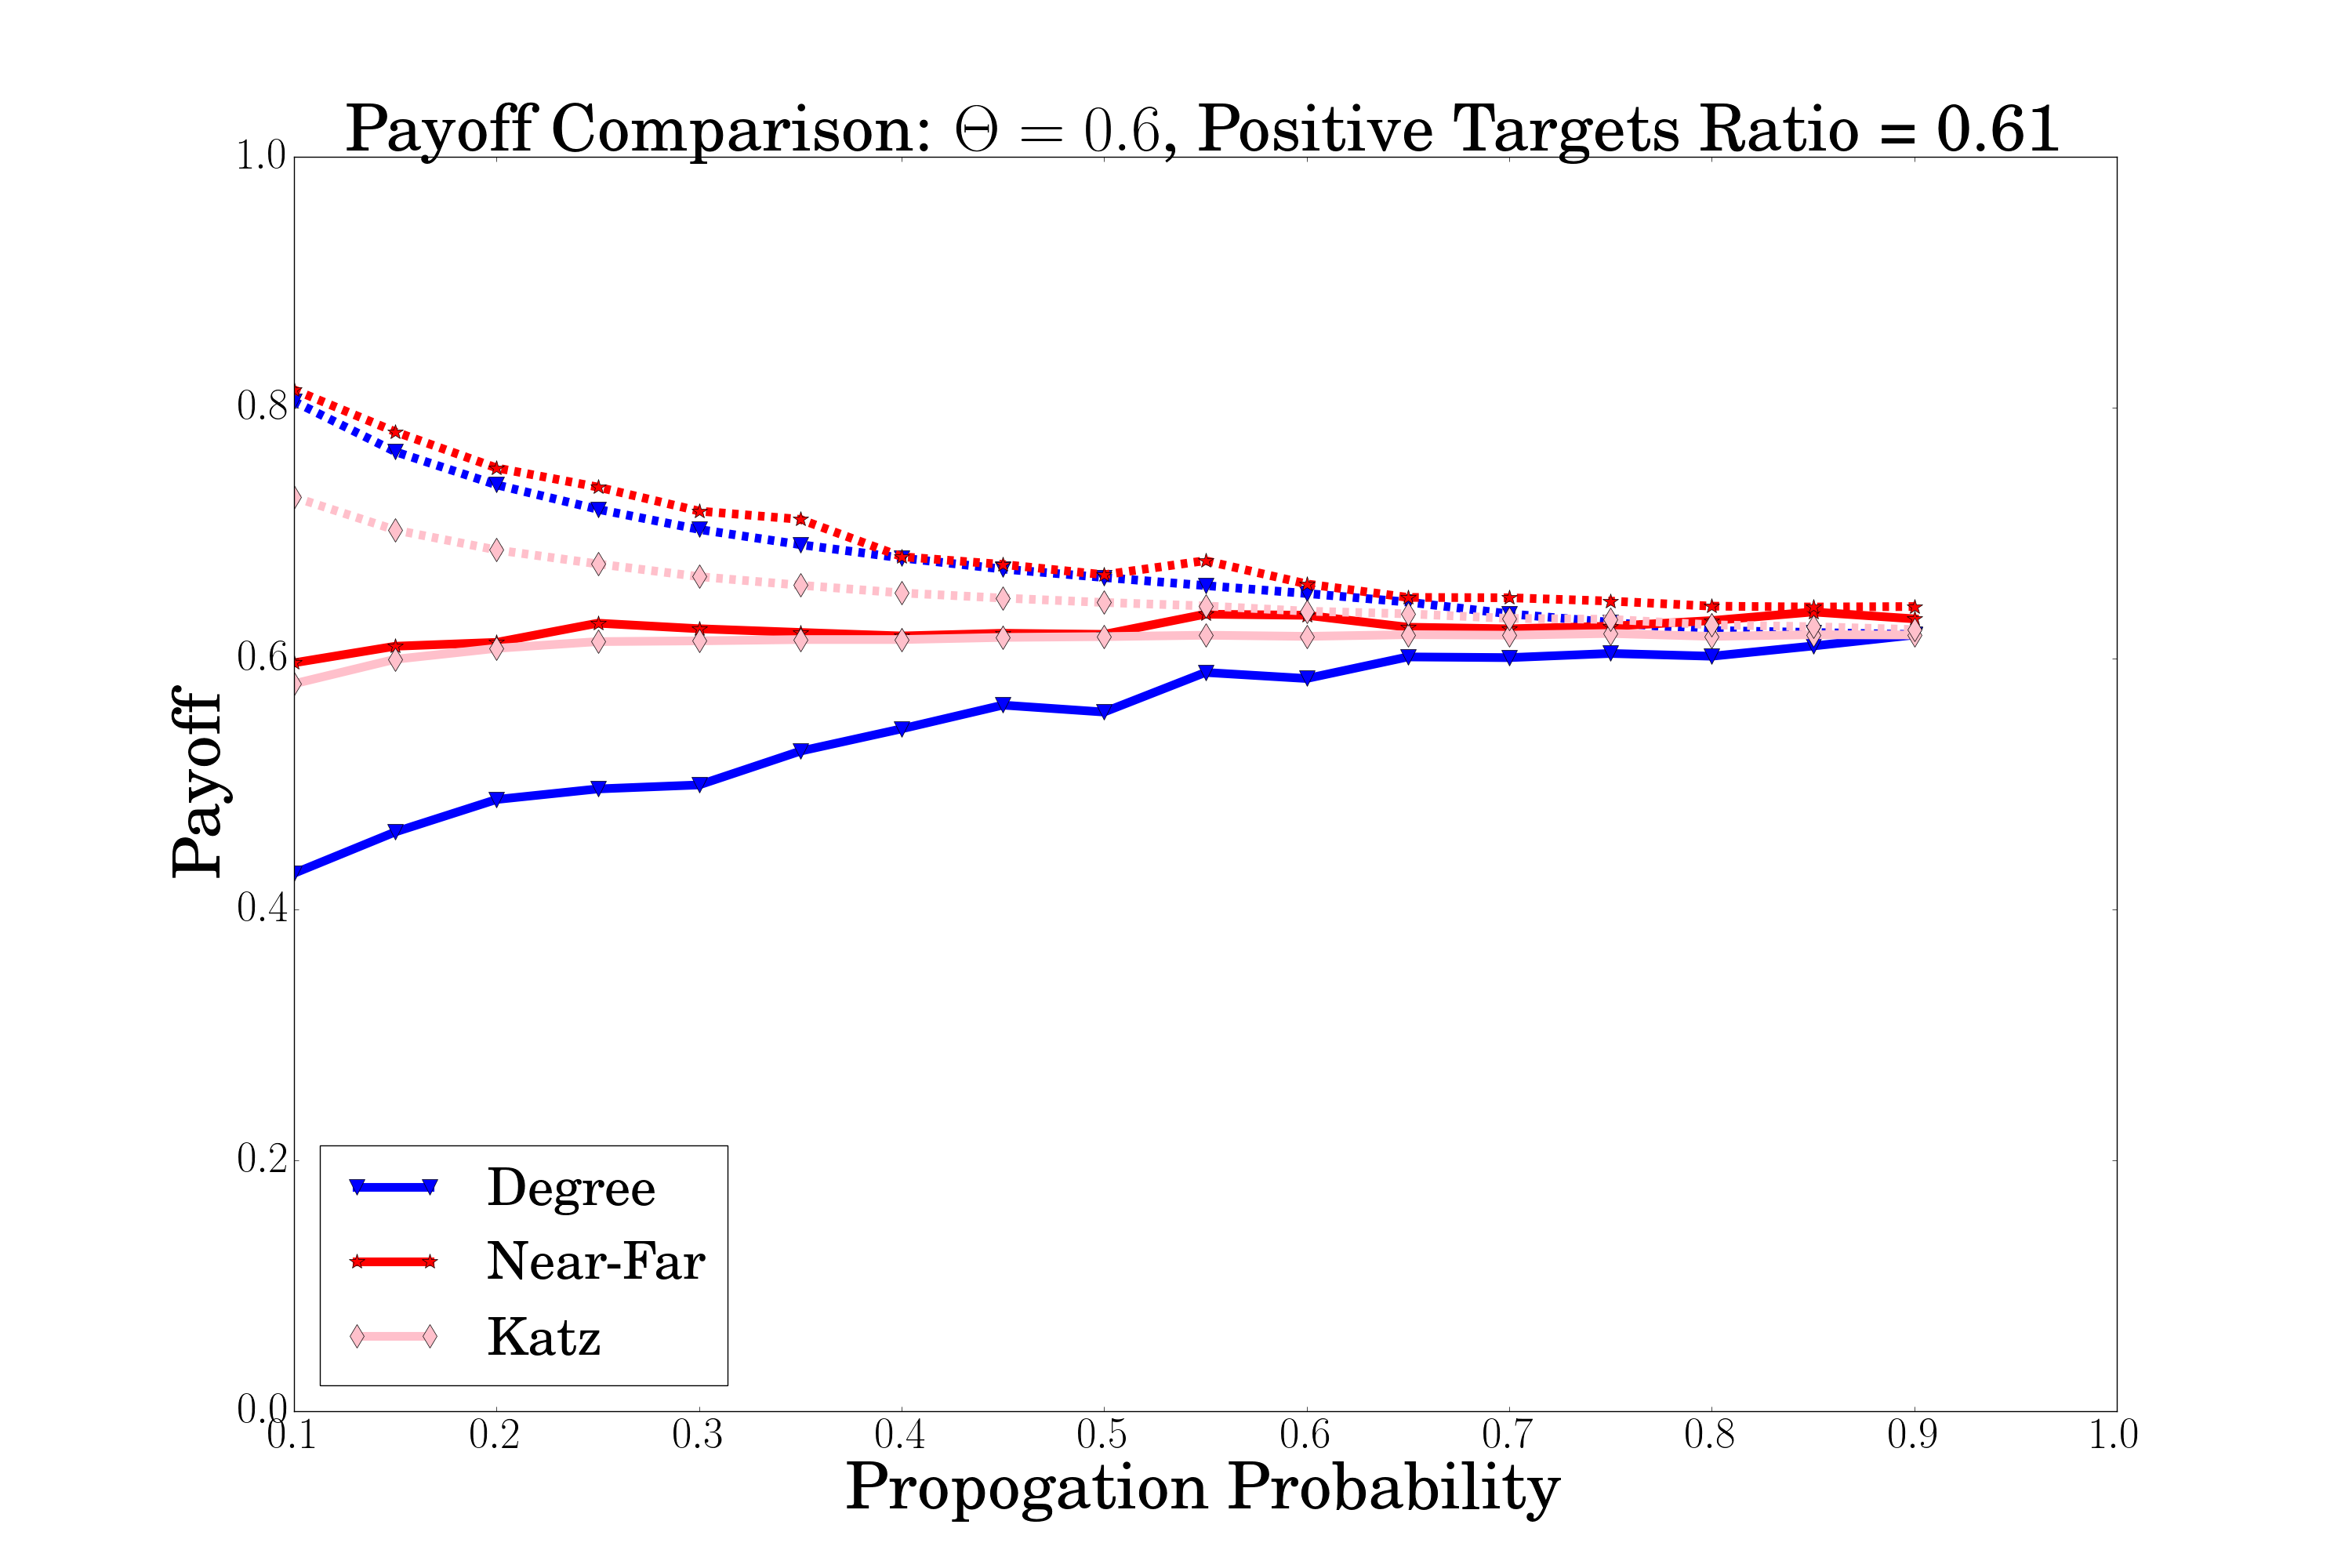
\includegraphics[width=1\textwidth]{../plots/comparison/theta=6.png}
  \end{subfigure}\par\medskip
  \begin{subfigure}{\linewidth}
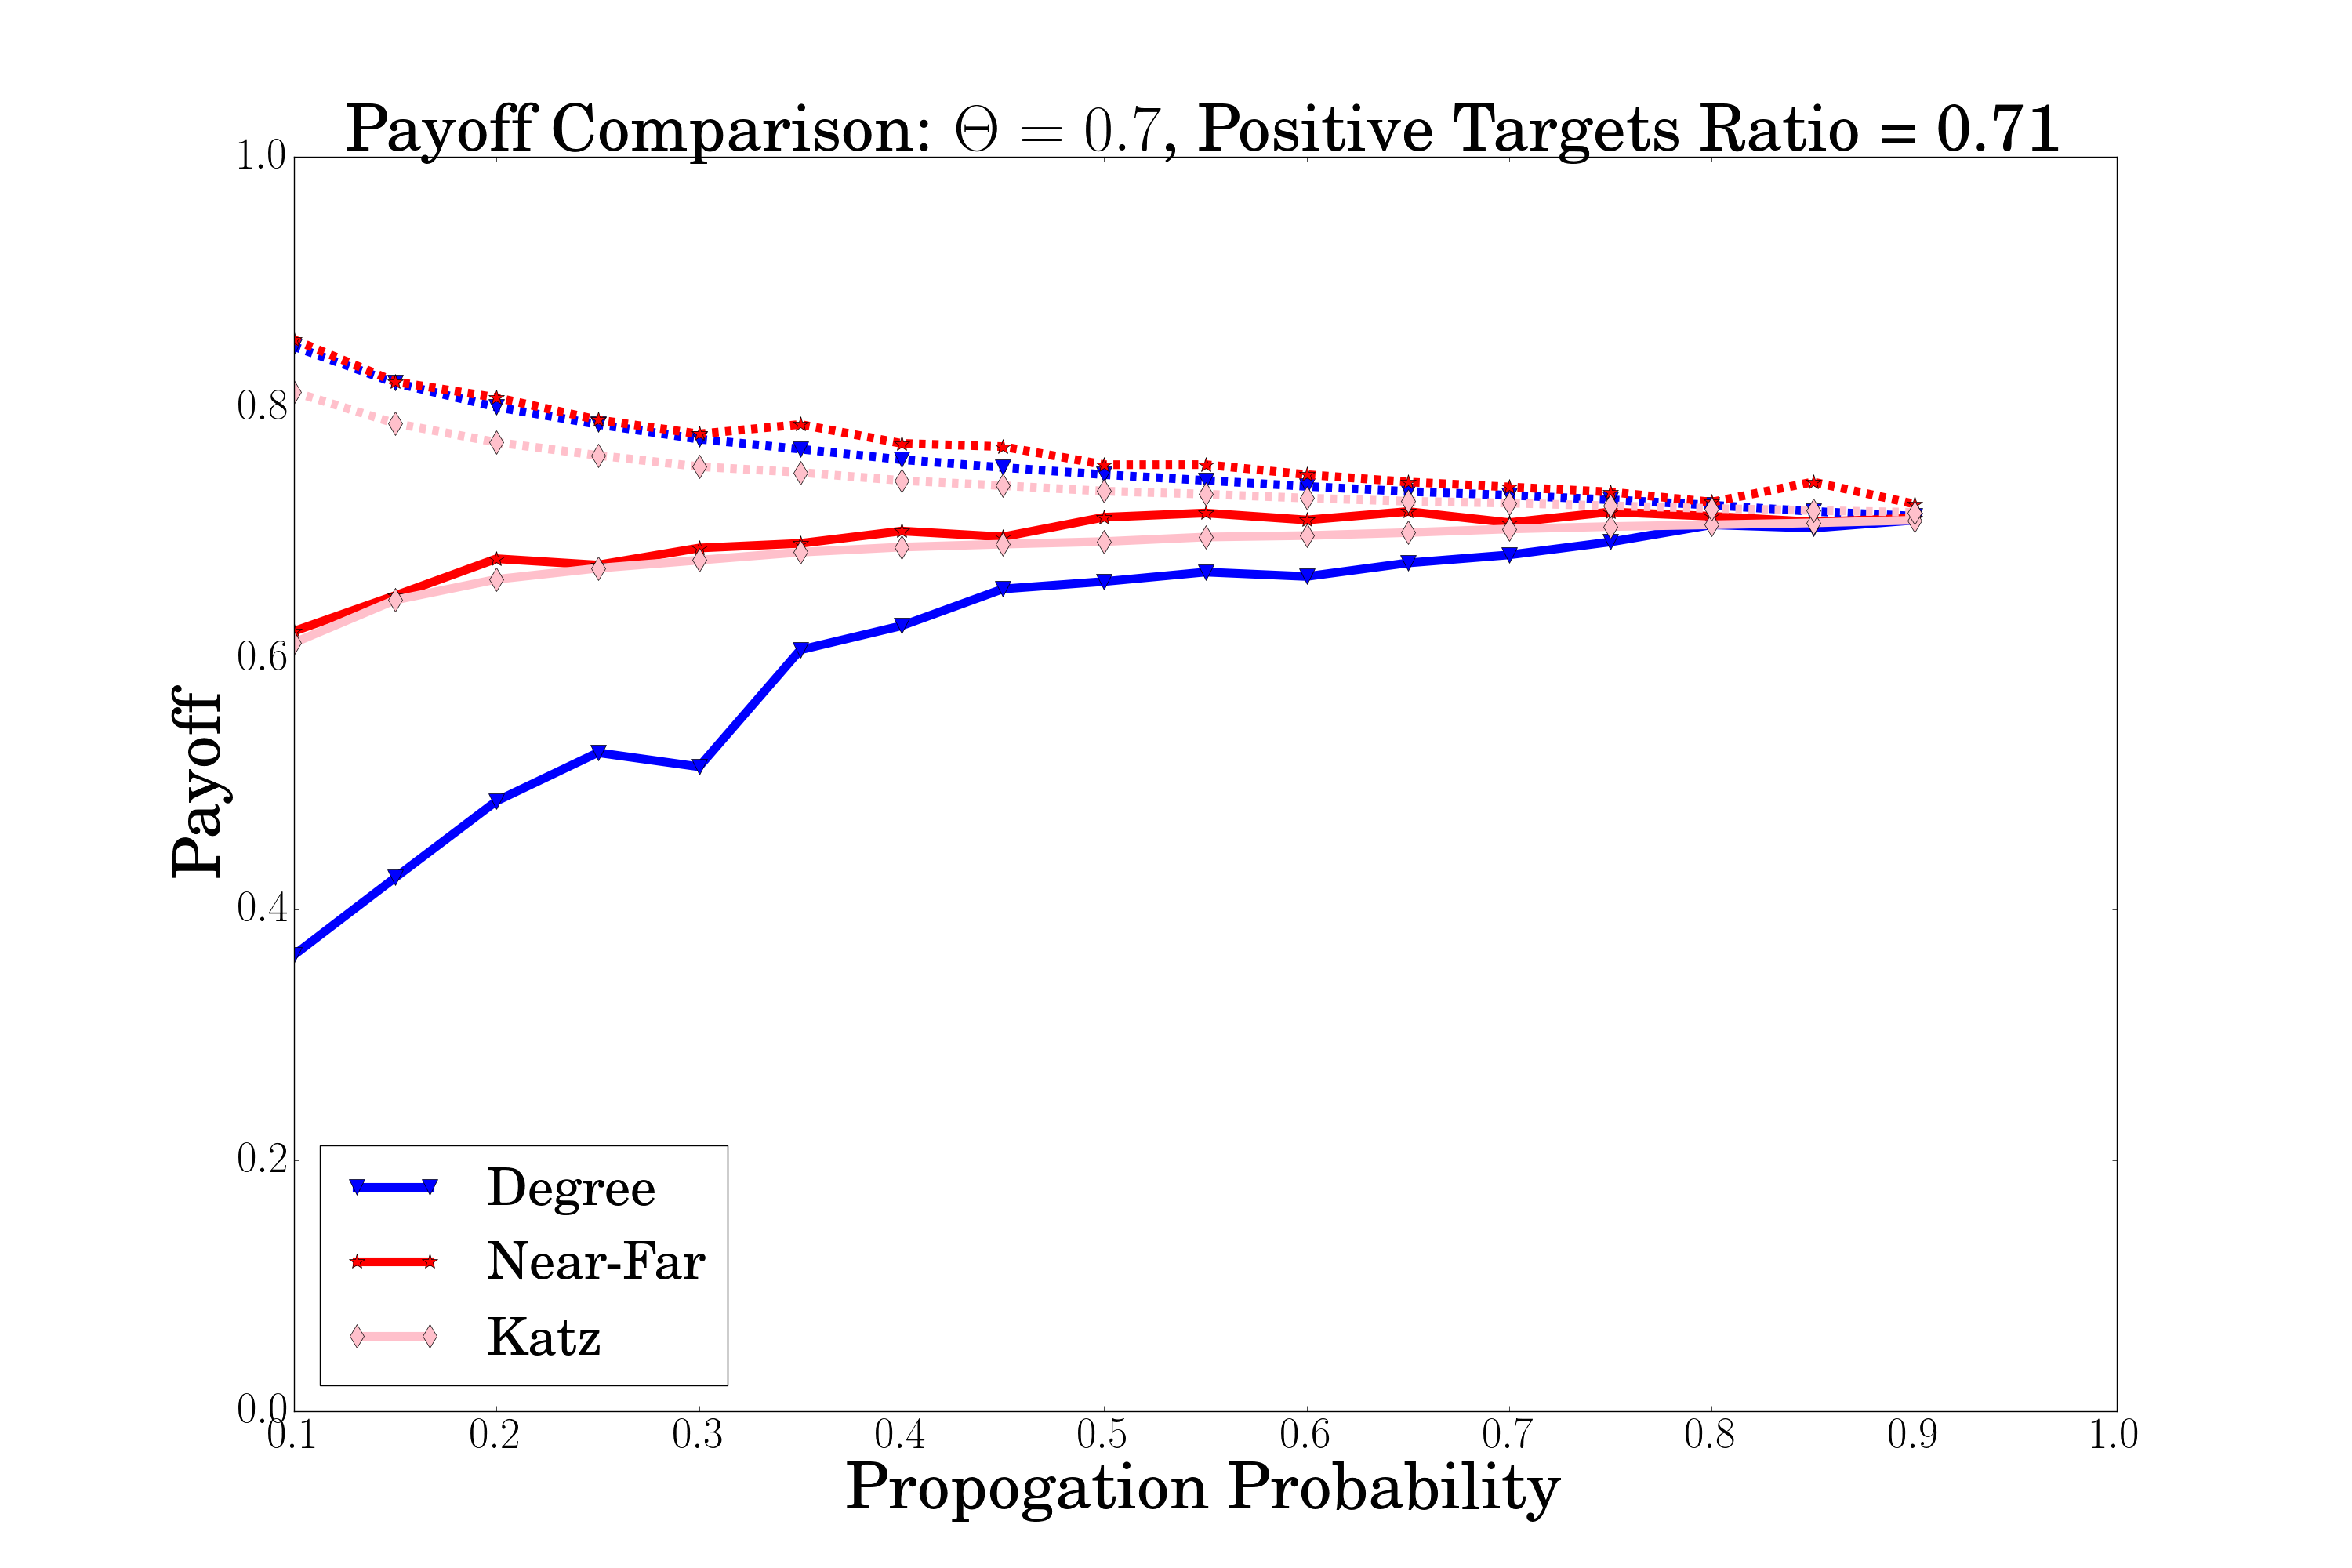
\includegraphics[width=1\textwidth]{../plots/comparison/theta=7.png}
  \end{subfigure}\par\medskip
  \caption{Comparison of Budgeted and Unbudgeted Results. Dashed lines are Unbudgeted scores.}
\end{figure}


\subsection{Key Observations of Budgeted Results}

Considering the plots presented in Figure 1, it is noticeable that the Farthest policy (Farthest from Negative) performs well when $\theta < 0.5$ and performs very poorly when $\theta > 0.5$. In contrast, the Betweenness policy performs well when $\theta > 0.5$ and performs very poorly when $\theta < 0.5$. These two policies show the limitations of too simple policies. Next we observe that the Near-Far policy outperforms all other policies regardless of the $\theta$ value and is less sensitive to it, highlighting the efficiency of the policy at the cost of simplicity. Finally, we see that there does seem to exist an inherent trade-off between simplicity and efficiency.

\textit{Farthest and Betweenness Performance}

From Figure 1, we see an interesting trend that the Farthest policy performs well when $\theta < 0.5$ and performs very poorly when $\theta > 0.5$ and the Betweenness policy is the exact opposite. Intuitively, this makes sense. The Farthest policy takes into account only the negative nodes, and tries to pick nodes that are as far away as possible, making it well suited for regimes when $\theta < 0.5$ as the majority of the nodes in the graph are negative target nodes. In contrast, the Betweenness policy takes into account only the positive nodes, and chooses the node with highest betweenness measure amongst the positive nodes, making it well suited for regimes when $\theta > 0.5$ as the majority of the nodes in the graph are positive target nodes. The performance of these two policies show the limitations of only considering either the positive or negative target nodes and exemplifies the cost in efficiency for simpler policies.

\textit{Near-Far Outperforms}

The Near-Far policy outperforms all other policies regardless of the $\theta$ and $p$ values, and can be seen in Figure 1. Further, it seems to be the only policy that is less sensitive to the $\theta$ value and performs well regardless. 

\textit{Simplicity and Efficiency Trade-off}

We saw earlier that the Farthest and Betweenness policies, while they utilize the computationally heavy distance metric, are still rather simplistic policies in the sense that they only consider either the positive or negative nodes. As a result, these policies can only handle one side of the spectrum of $\theta$ values and performs poorly on the other. The Degree policy, in contrast, considers both the positive and negative nodes, but does not perform any distance metric calculations, once again making it simplistic. As a result, we see that the Degree policy performs mediocrely across all $\theta$ values. Finally, we see that with the Near-Far policy, which considers both the positive and negative nodes, and also utilizes the distance metric is a more complex policy and proves to outperform under all regimes. These results highlight the inherent trade-off between simplicity and efficiency within the policies. As we sacrifice information and calculations, we have a more simplistic policy but at the cost of efficiency.

\subsection{Key Observations of Unbudgeted Comparison}

Considering the plots presented in Figure 2, we see that when $\theta < 0.5$, all policies but the Near-Far performs very poorly in the unbudgeted regime, exemplifying the Near-Far's superior efficiency. When $\theta > 0.5$, we see the scores are more similar, but the trend of Near-Far outperforming all other policies still remains. Finally, looking at Figure 3 that compares the scores in the budgeted and unbudgeted regime,  we see that the Near-Far policy performs better when unbudgeted. The other policies; however, perform better in the budgeted regime when $\theta < 0.5$.

\textit{ Near-Far Outperforms}

The similar trend that Near-Far outperforms all other policies can be seen in the unbudgeted regime. This is especially obvious when $\theta < 0.5$ and still prevalent when $\theta > 0.5$. At first glance, one might think that this is because many of the policies besides Near-Far pick $(1-p)*|V^+_\theta|$ seed nodes. Intuitively, it is natural that when $\theta < 0.5$, there are more negative nodes, and thus enforcing one to pick many seed nodes forces the policies to be bad, while when $\theta > 0.5$ this is not a problem. However, the Katz policy, like Near-Far, does not have this restriction and still performs poorly. This shows that the Near-Far policy is actually good at handling the unbudgeted regime and choosing only necessary seed nodes.

\textit{Unbudgeted vs. Budgeted}

From Figure 3, we see that the Near-Far policy is able to take advantage of the unbudgeted regime and always performs better than when it is budgeted, regardless of the $\theta$ value. Besides the Near-Far policy, we see the general trend that the policies score higher in the unbudgeted regime only when $\theta > 0.5$ and worse when $\theta < 0.5$. This makes sense, as the other policies are not good at choosing only necessary seeds. Thus, when $\theta > 0.5$ and there are more positive nodes, the unbudgeted regime is able to perform better, while it underperforms in the $\theta < 0.5$ setting.


